%---------------------------------------------------------------------
%
% Chapter 7: Empirical Analysis On Road Map Problems
%
%---------------------------------------------------------------------
%
% ChapEmpiricalAnalysisRoadMaps.tex
% Copyright 2015 Dr. Francisco J. Pulido
%
% This file belongs to the PhD titled "New Techniques and Algorithms for Multiobjective and Lexicographic Goal-Based Shortest Path Problems", distributed under the Creative Commons Licence Attribution-NonCommercial-NoDerivs 3.0, available in http://creativecommons.org/licenses/by-nc-nd/3.0/. The complete PhD dissertation is freely accessible from http://www.lcc.uma.es/~francis/
%
% This thesis has been written adapting the TeXiS template, a LaTeX template for writting thesis and other documents. The complete TeXiS package can be obtained from http://gaia.fdi.ucm.es/projects/texis/. TeXis is distributed under the same conditions of the LaTeX Project Public License (http://www.latex-project.org/lppl.txt). The complete license is available in http://creativecommons.org/licenses/by-sa/3.0/legalcode
%
%---------------------------------------------------------------------

\chapter{Empirical Analysis On Road Map Problems}
\label{chapEmpiricalAnalysisRoadMaps}
%
\begin{FraseCelebre}
\begin{Frase}
The rise of Google, the rise of Facebook, the rise of Apple, I think are proof that there is a place for computer science as something that solves problems that people face every day.
\end{Frase}
\begin{Fuente}
Eric Schmidt (1955-)
\end{Fuente}
\end{FraseCelebre}
%
%\begin{resumen}
%

This chapter is devoted to analyze the algorithmic performance on realistic road maps from the "9th DIMACS Implementation Challenge: Shortest Path". The challenge comprises a set of twelve road maps of increasing size. In particular, we use the New York city map. Additionally we have employed a second road map from the UA Census 2000 TIGER/Line Files, which was assembled by Dr. Dominik Schultes\footnote{<mail@dominik-schultes.de>} and is available from the same site. In particular, we use the Vermont State map.

All DIMACS maps provide two different cost values: \textit{physical distance} and \textit{travel time}. An additional cost was introduced in \cite{Machuca2011} by calculating the \textit{travel economic cost}. This was obtained combining tolls and fuel consumption according to road category. The resulting values are not linearly correlated to those of the other cost values. The experiments reported below consider the simultaneous minimization of these three attributes, physical distance $(c_1)$, travel time $(c_2)$, and travel economic cost $(c_3)$ (further details about these experiments can be seen in  Section \ref{chapMultiObjTestBeds:subsec:RoadMaps}). 

The two maps selected for our experiments have different sizes. Table \ref{tab:7-1} shows the coordinates and number of nodes and arcs for each map. The NY city map represents a difficult problem to be tackled with three objectives and only some problems could be solved. The other map, VT$_{cut}$, corresponds to a trimmed version of the original map of Vermont, reduced to approximately 70\% of its original size in order to allow the solution of the complete set of experiments by all the algorithms. Renderings of the NY and VT$_{cut}$ maps are presented in Figures \ref{fig:7-1} and \ref{fig:7-2}, respectively.

\begin{table}
\caption{Maps employed in the road map experiments. ($^*$) corresponds to a cut of the original map.}
\label{tab:7-1}
\begin{center}
\begin{tabular}{ccrrrr}
\hline \noalign{\smallskip} 
Description & Acronym & Nodes & Arcs & Longitude & Latitude \\
\noalign{\smallskip} \hline 
New York city& NY & 264,346 & 730,100 & [73.5-74.5]$^{\circ}$W & [40.3-41.3]$^{\circ}$N \\
%New York city* & NY(2) & 79,754 & 210,974 & [74-74.5]$^{\circ}$W & [40.7-41.3]$^{\circ}$N \\
Vermont State$^*$ & VT$_{cut}$ & 69,575 & 152,012 & [72-73.5]$^{\circ}$W & [43.5-45.0]$^{\circ}$N \\
%Delaware State & DE & 49,109 & 119,744 & [75-75.8]$^{\circ}$W & [38.4-40.0]$^{\circ}$N \\
\hline
\end{tabular} 
\end{center}
\end{table}

\begin{figure}[ht] 
  \begin{minipage}[b]{0.45\linewidth}
    \centering
    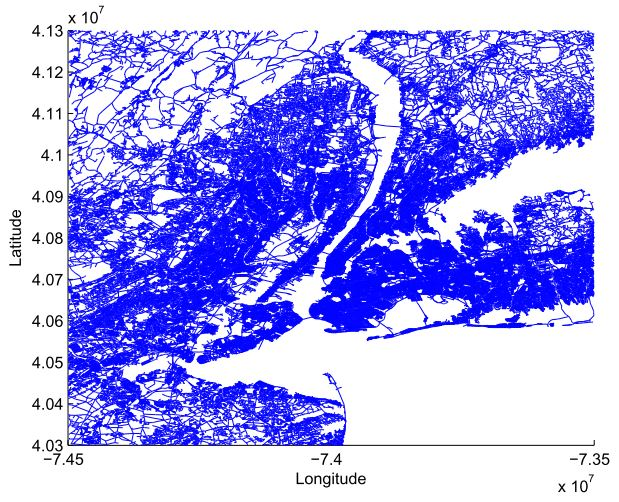
\includegraphics[width=1\linewidth]{Images/Chapter7/NY} 
    \caption{Rendering of NY city map} 
    \label{fig:7-1} 
    %\vspace{4ex}
  \end{minipage}%%
\hspace{5mm}
  \begin{minipage}[b]{0.45\linewidth}
    \centering
    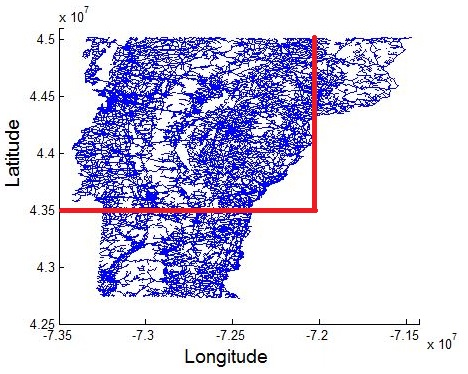
\includegraphics[width=1\linewidth]{Images/Chapter7/VTcut} 
    \caption{Cut of Vermont map (squared)} 
	 \label{fig:7-2}
	%\vspace{4ex}
  \end{minipage} 
\end{figure}

We selected the first twenty problems for the New York city road map proposed in \cite{Machuca2012}. These problems were randomly generated using an uniform distribution to select start and destination nodes. In a similar manner, we generated twenty random problems for the VT$_{cut}$ map. These test sets and the additional generated map files are available online\footnote{http://alef.iaia.lcc.uma.es/projects/alef-public/wiki/Benchmarks}. 
%Only algorithms \namoate \ and \namoalin \ are reported over these sets, since \namoalin \ clearly outperforms \namoalex.

Since previously reported runtimes of \namoa \ solving a biobjective version of these problems (minimizing  $c_2$ and $c_3$, i.e. much easier problems) were up to several days \citep{Machuca2011a}, we also established a runtime limit of 8 hours for the experiments over the NY city map. 

The algorithms were implemented in Common Lisp using LispWorks Professional 6.01 (64-bit), and run on a Sun Fire X4140 server with 2 six-core AMD Opteron 2435 at 2.60 GHz processors and 64 GB of DDR2 RAM memory. This machine is slower than the one employed to solve the random grid experiments, however, it was chosen due to the greater memory space requirements of the problem analyzed here. All experiments were run on a single thread.

In the following, we conduct an experimental evaluation of the algorithms in an analogous fashion of that performed in Chapter \ref{chapEmpiricalAnalysisGrids} for random grid problems.

%-------------------------------------------------------------------
\section{\texorpdfstring{\lexgo}{LEXGO*} \ vs \texorpdfstring{\namoa}{NAMOA*}}
\label{chapEmpiricalAnalysis:sec:resultsdimacslexgo}
%-------------------------------------------------------------------

This section analyzes \namoa \ and \lexgo on the realistic road maps of Vermont and New York city. The study is applied to the lexicographic and linear selection orders (see Definitions \ref{chapMultiObjAlg:def:lexorder} and \ref{chapMultiObjAlg:def:linorder} for further description), and performed over the two classes of experiments already described for random grids in Section \ref{chapEmpiricalAnalysis:sec:grids}.

The full set of experiments on Vermont was solved by all the algorithms, however, out of the twenty problems which compose the problem set of New York city, \namoalex \ and \namoalin \ were capable of solving only four of them, NY\#2, NY\#4, NY\#5 and NY\#16. The comparison to their \lexgo \ counterpart using the same selection order follows.
 
%-------------------------------------------------------------------
\subsection{Analysis on class I experiments}
\label{chapEmpiricalAnalysis:subsec:analysisdimacslexgoc1}
%-------------------------------------------------------------------

Target values for \lexgo \ were defined as in Equation \ref{eq:targets} for random grids class I experiments. Table \ref{tab:7-2} displays the percentage of goal-optimal solution vectors returned by \lexgo \ relative to the full set ($C^*$) returned by \namoa. 

\begin{table}
\caption{Class I experiments in road maps, percentage of goal-optimal solution vectors relative to $C^*$ for solvable problems within the time limit by \lexgo \ and \namoa. An asterisk ($^*$) indicates that the goals could not be satisfied.}
\label{tab:7-2}
\centering
\begin{tabular}{crrrrrrrr}
\hline \noalign{\smallskip}
& & & \multicolumn{5}{c}{\lexgo} \\
\noalign{\smallskip} \cline{4-8} \noalign{\smallskip}
& & \namoa & 1 & 0.75 & 0.5 & 0.25 & 0 & $k_1$\\
\noalign{\smallskip} 
 & $n$ & $|C^*|$ & \% & \% & \% & \% & \% & \\
\cline{1-8} \noalign{\smallskip} 
\parbox[t]{2mm}{\multirow{20}{*}{\rotatebox[origin=c]{90}{Vermont}}} & 1 & 1,252 & 100 & 3.04 & 0.64 & $^*$0.08 & $^*$0.08 \\
& 2 & 223 & 100 & 38.57 & 34.53 & $^*$0.45 & $^*$0.45 \\
& 3 & 34 & 100 & 67.65 & 29.41 & $^*$2.94 & $^*$2.94 \\
& 4 & 4,759 & 100 & 57.11 & 17.42 & $^*$0.02 & $^*$0.02 \\
& 5 & 334 & 100 & 36.23 & 1.80 & $^*$0.30 & $^*$0.30 \\
& 6 & 7,576 & 100 & 84.52 & 19.97 & $^*$0.01 & $^*$0.01 \\
& 7 & 3 & 100 & 33.33 & $^*$33.33 & $^*$33.33 & $^*$33.33 \\
& 8 & 5 & 100 & 60.00 & 20.00 & $^*$20.00 & $^*$20.00 \\
& 9 & 206 & 100 & 47.09 & 23.30 & $^*$0.49 & $^*$0.49 \\
& 10 & 9,712 & 100 & 82.22 & 20.15 & $^*$0.01 & $^*$0.01 \\
& 11 & 14,537 & 100 & 54.95 & 48.81 & $^*$0.01 & $^*$0.01 \\
& 12 & 1,648 & 100 & 32.52 & $^*$0.06 & $^*$0.06 & $^*$0.06 \\
& 13 & 10,256 & 100 & 92.82 & 43.80 & $^*$0.01 & $^*$0.01 \\
& 14 & 444 & 100 & 55.41 & 21.17 & $^*$0.23 & $^*$0.23 \\
& 15 & 1,310 & 100 & 49.16 & 4.81 & $^*$0.08 & $^*$0.08 \\
& 16 & 1,216 & 100 & 1.64 & $^*$0.08 & $^*$0.08 & $^*$0.08 \\
& 17 & 8,189 & 100 & 58.30 & 23.70 & $^*$0.01 & $^*$0.01 \\
& 18 & 38 & 100 & 65.79 & 18.42 & $^*$2.63 & $^*$2.63 \\
& 19 & 1 & 100 & 100.00 & 100.00 & 100.00 & 100.00 \\
& 20 & 4,949 & 100 & 33.97 & 9.23 & $^*$0.02 & $^*$0.02 \\
\noalign{\medskip}
\parbox[t]{2mm}{\multirow{4}{*}{\rotatebox[origin=c]{90}{NY city}}} & 2 & 303 & 100 & 57.42 & 4.62 & $^*$0.33 & $^*$0.33 \\
& 4 & 4,429 & 100 & 88.82 & 74.32 & $^*$0.02 & $^*$0.02 \\
& 5 & 7 & 100 & 71.42 & $^*$14.28 & $^*$14.28 & $^*$14.28 \\
& 16 & 1,640 & 100 & 48.35 & $^*$0.06 & $^*$0.06 & $^*$0.06 \\
\hline
\end{tabular}
\end{table}

Table \ref{tab:7-3} shows the relative percentage number of scanned labels by \lexgolin \ to \namoalin in Vermont and NY city maps. As it was mentioned before, the number of explored labels by \namoalin \ is nearly the same as \namoalex. This slight difference is attributed to the \emph{lazy filtering} procedure applied to both alternatives. This is also the case of \lexgolex \ and \lexgolin.

\begin{table}
\caption{Class I experiments in road maps, relative percentage number of scanned labels by \lexgolin \ to \namoalin.}
\label{tab:7-3}
\centering
\begin{tabular}{crrrrrrrr}
\hline \noalign{\smallskip}
& & & \multicolumn{5}{c}{\lexgolin} \\
\noalign{\smallskip} \cline{4-8} \noalign{\smallskip}
& & \namoalin & 1 & 0.75 & 0.5 & 0.25 & 0 & \multicolumn{1}{c}{$k_1$}\\
\noalign{\smallskip} 
 & $n$ & $\sum G_{cl}$ & \% & \% & \% & \% & \% & \\
\cline{1-8} \noalign{\smallskip} 
\parbox[t]{2mm}{\multirow{20}{*}{\rotatebox[origin=c]{90}{Vermont}}} & 1 & 211,268 & 99.73 & 46.80 & 11.63 & 4.05 & 0.07 \\ 
& 2 & 115,435 & 99.99 & 50.41 & 43.08 & 17.81 & 0.44 \\ 
& 3 & 11,332 & 96.86 & 83.15 & 49.28 & 15.91 & 2.06 \\ 
& 4 & 1,134,467 & 99.99 & 80.17 & 32.35 & 2.95 & 0.03 \\ 
& 5 & 45,650 & 96.65 & 72.95 & 16.58 & 3.59 & 1.65 \\ 
& 6 & 5,497,553 & 99.17 & 93.42 & 44.25 & 2.88 & 0.01 \\ 
& 7 & 187 & 73.26 & 55.61 & 55.08 & 57.75 & 45.99 \\ 
& 8 & 480 & 88.33 & 61.46 & 33.96 & 22.29 & 22.08 \\ 
& 9 & 65,140 & 99.76 & 67.24 & 39.98 & 15.10 & 0.71 \\ 
& 10 & 5,332,256 & 98.31 & 86.29 & 33.43 & 9.20 & 0.02 \\ 
& 11 & 10,125,074 & 98.27 & 72.55 & 69.46 & 19.64 & 0.02 \\ 
& 12 & 127,611 & 97.45 & 29.81 & 5.49 & 3.33 & 0.54 \\ 
& 13 & 8,664,536 & 99.98 & 97.45 & 70.83 & 20.19 & 0.01 \\ 
& 14 & 47,215 & 99.30 & 76.21 & 34.57 & 4.91 & 0.19 \\ 
& 15 & 571,195 & 99.95 & 93.83 & 68.61 & 3.35 & 0.21 \\ 
& 16 & 88,699 & 96.76 & 47.69 & 33.91 & 20.55 & 0.44 \\ 
& 17 & 1,223,581 & 99.60 & 73.43 & 26.25 & 4.96 & 0.16 \\ 
& 18 & 11,021 & 76.33 & 52.55 & 36.53 & 13.51 & 2.79 \\ 
& 19 & 92 & 64.13 & 64.13 & 64.13 & 64.13 & 64.13 \\ 
& 20 & 1,904,080 & 99.99 & 71.65 & 39.55 & 11.26 & 0.03 \\
\noalign{\medskip}
\parbox[t]{2mm}{\multirow{4}{*}{\rotatebox[origin=c]{90}{NY city}}} &
2 & 17,294 & 93.96 & 61.91 & 17.83 & 2.80 & 3.64 \\
& 4 & 3,390,656 & 99.40 & 92.23 & 74.00 & 9.14 & 0.01 \\
& 5 & 719 & 47.98 & 32.96 & 10.43 & 6.53 & 8.20 \\
& 16 & 2,445,191 & 81.14 & 47.17 & 11.67 & 0.53 & 0.01 \\ 
\hline
\end{tabular}
\end{table}

Finally, Tables \ref{tab:7-4} and \ref{tab:7-5} display the runtimes of \namoa \ and the relative time of \lexgo \ to \namoa \ for the maps of Vermont and NY city with the lexicographic and linear selection orders, respectively. When the runtime of \namoa \ was smaller than 0.01 seconds, we display $<0.01$ in the tables, and complete the relative percentages of \lexgo \ with dashes to indicate that those are not significative. Likewise, if the relative percentage of runtime of \lexgo \ to \namoa \ was smaller than 0.01\%, we simply display $<0.01$.

\begin{table}
\caption{Class I experiments in road maps, relative percentage runtimes in seconds for \lexgolex \ and \namoalex.}
\label{tab:7-4}
\centering
\begin{tabular}{crrrrrrrr}
\hline \noalign{\smallskip}
& & & \multicolumn{5}{c}{\lexgolex} \\
\noalign{\smallskip} \cline{4-8} \noalign{\smallskip}
& & \namoalex & 1 & 0.75 & 0.5 & 0.25 & 0 & \multicolumn{1}{c}{$k_1$}\\
\noalign{\smallskip} 
 & $n$ & Runtime (s) & \% & \% & \% & \% & \% & \\
\cline{1-8} \noalign{\smallskip} 
\parbox[t]{2mm}{\multirow{20}{*}{\rotatebox[origin=c]{90}{Vermont}}} & 1 & 39.95 & 106.68 & 16.20 & 3.12 & 1.21 & 0.04 \\ 
& 2 & 7.05 & 118.81 & 41.81 & 32.29 & 18.81 & 0.67 \\ 
& 3 & 0.32 & 137.80 & 117.18 & 58.43 & 18.90 & <0.01 \\ 
& 4 & 1,386.53 & 99.14 & 59.88 & 7.81 & 0.28 & <0.01 \\ 
& 5 & 2.49 & 111.26 & 66.23 & 22.52 & 2.48 & 2.52 \\ 
& 6 & 17,731.38 & 95.35 & 76.09 & 12.22 & 0.18 & <0.01 \\ 
& 7 & <0.01 & - & - & - & - & - \\ 
& 8 & <0.01 & - & - & - & - & - \\ 
& 9 & 3.60 & 121.23 & 61.48 & 28.56 & 16.46 & 0.42 \\ 
& 10 & 17,828.99 & 100.05 & 73.27 & 6.57 & 1.62 & <0.01 \\ 
& 11 & 30,318.76 & 99.85 & 57.99 & 47.17 & 2.77 & <0.01 \\ 
& 12 & 40.21 & 97.90 & 11.09 & 1.09 & 0.85 & 0.04 \\ 
& 13 & 29,337.51 & 104.79 & 97.68 & 38.46 & 7.92 & <0.01 \\ 
& 14 & 3.83 & 102.84 & 68.71 & 26.81 & 3.26 & <0.01 \\ 
& 15 & 115.33 & 102.54 & 83.58 & 42.54 & 0.78 & 0.03 \\ 
& 16 & 8.54 & 94.53 & 18.61 & 18.25 & 8.57 & <0.01 \\ 
& 17 & 2,245.32 & 96.76 & 44.88 & 5.07 & 0.39 & <0.01 \\ 
& 18 & 0.34 & 104.66 & 113.70 & 40.82 & 18.37 & <0.01 \\ 
& 19 & <0.01 & - & - & - & - & - \\ 
& 20 & 1,899.15 & 95.95 & 33.55 & 7.18 & 2.23 & <0.01 \\
\noalign{\medskip}
\parbox[t]{2mm}{\multirow{4}{*}{\rotatebox[origin=c]{90}{NY city}}} &
2 & 1.48 & 97.97 & 54.72 & 15.54 & 0.67 & 0.67 \\
& 4 & 4,752.77 & 101.94 & 84.97 & 59.52 & 1.57 & <0.01 \\
& 5 & <0.01 & - & - & - & - & - \\
& 16 & 559.76 & 81.93 & 41.86 & 11.30 & 0.18 & <0.01 \\
\hline
\end{tabular}
\end{table}

\begin{table}
\caption{Class I experiments in road maps, relative percentage runtimes in seconds for \lexgolin \ and \namoalin.}
\label{tab:7-5}
\centering
\begin{tabular}{crrrrrrrr}
\hline \noalign{\smallskip}
& & & \multicolumn{5}{c}{\lexgolin} \\
\noalign{\smallskip} \cline{4-8} \noalign{\smallskip}
& & \namoalin & 1 & 0.75 & 0.5 & 0.25 & 0 & \multicolumn{1}{c}{$k_1$}\\
\noalign{\smallskip} 
 & $n$ & Runtime (s) & \% & \% & \% & \% & \% & \\
\cline{1-8} \noalign{\smallskip} 
\parbox[t]{2mm}{\multirow{20}{*}{\rotatebox[origin=c]{90}{Vermont}}} &
1 & 40.02 & 98.71 & 20.78 & 4.80 & 1.29 & 0.04 \\ 
& 2 & 7.35 & 125.05 & 47.35 & 42.46 & 22.71 & 0.22 \\ 
& 3 & 0.30 & 194.93 & 166.66 & 94.59 & 26.35 & 5.41 \\ 
& 4 & 1,428.44 & 88.94 & 55.66 & 7.46 & 0.33 & <0.01 \\ 
& 5 & 2.62 & 136.28 & 97.02 & 19.65 & 2.40 & 1.18 \\ 
& 6 & 17,913.28 & 90.27 & 77.75 & 12.81 & 0.19 & <0.01 \\ 
& 7 & <0.01 & - & - & - & - & - \\ 
& 8 & <0.01 & - & - & - & - & - \\ 
& 9 & 3.42 & 131.02 & 73.95 & 45.22 & 21.45 & 0.91 \\ 
& 10 & 17,167.54 & 100.51 & 70.97 & 8.03 & 1.83 & <0.01 \\ 
& 11 & 28,712.69 & 96.00 & 52.18 & 42.35 & 3.83 & <0.01 \\ 
& 12 & 39.25 & 106.76 & 12.44 & 1.31 & 0.60 & 0.20 \\ 
& 13 & 27,556.06 & 101.59 & 95.62 & 34.33 & 9.40 & <0.01 \\ 
& 14 & 3.88 & 127.32 & 91.99 & 35.35 & 4.02 & <0.01 \\ 
& 15 & 108.65 & 102.89 & 93.65 & 60.95 & 1.38 & 0.04 \\ 
& 16 & 7.64 & 109.59 & 28.98 & 21.23 & 15.50 & 0.20 \\ 
& 17 & 2,077.78 & 100.42 & 51.94 & 5.04 & 0.48 & <0.01 \\ 
& 18 & 0.52 & 93.79 & 96.89 & 45.44 & 12.23 & 3.11 \\ 
& 19 & <0.01 & - & - & - & - & - \\ 
& 20 & 1,699.91 & 104.33 & 29.30 & 9.66 & 2.87 & <0.01 \\ 
\noalign{\medskip}
\parbox[t]{2mm}{\multirow{4}{*}{\rotatebox[origin=c]{90}{NY city}}} &
2 & 1.43 & 129.37 & 86.01 & 25.87 & 2.09 & 0.69 \\
& 4 & 3,963.98 & 110.34 & 105.57 & 85.97 & 4.35 & <0.01 \\
& 5 & <0.01 & - & - & - & - & - \\
& 16 & 712.59 & 71.32 & 52.04 & 11.02 & 0.14 & <0.01 \\
\hline
\end{tabular}
\end{table}

The results obtained for the road map problems are much more heterogeneous than the ones for random grids. Thus, we can observe a wide range of goal-optimal solution ratios, for instance, the range of ratios of goal-optimal solution vectors returned for $k_1 = 0.75$ varies from 1.64\% to 92.82\% (see Table \ref{tab:7-2}) for Vermont map problems (VT\#16 and VT\#13, respectively). This could be expected, since the road map experiments represent a realistic scenario, on the contrary, the random grids were generated using an uniform distribution. However, both scenarios share the inability to satisfy the goals when $k_1 = 0.25$ or $k_1 = 0$.

The heterogeneity of the results remains regarding the labels scanned and the runtime of \lexgo, however, it shall be noticed that the runtime comparison between \namoalex \ and \namoalin \ does not show a clear advantage to \namoalin, as it happens in the grids experiments. 

Regarding the lexicographic order, \lexgo \ does perform in a very similar manner for the road maps as for the random grids. \lexgo \ explores for the most difficult problem solved by both algorithms, VT\#11 of Vermont, 98.27\%, 72.55\% and 69.46\% of the labels explored by \namoa \ for $k_1=1$, $k_1=0.75$ and $k_1=0.5$, respectively. 

The small time overhead observed in grid experiments for $k_1=1$ is also found in some of the road map experiments, as well as the important reductions in labels scanned and runtimes when $k_1 = 0.25$ or $k_1 = 0$, regardless the function employed as selection order.

We will further analyze in depth these data and the class II experiments reported below in the summary section. 

%-------------------------------------------------------------------
\subsection{Analysis on class II experiments}
\label{chapEmpiricalAnalysis:subsec:analysisdimacslexgoc2}
%-------------------------------------------------------------------

In the second class of experiments, goal preferences and target values were defined using $k_1 = \{0.75 , 0.5\}$ with all possible values of $k_2$ defined in Equation \ref{eq:targets2}. Tables \ref{tab:7-6} displays the relative number of goal-optimal solution vectors to the full Pareto set. The number of scanned labels for these maps is shown in Table \ref{tab:7-7}. Finally, Tables \ref{tab:7-8} and \ref{tab:7-9} show runtimes of \lexgo \ and \namoa \ with lexicographic and linear selection orders, respectively.

There are several cases where the solution returned is exactly the same. When problems NY\#5 and NY\#16 are solved with $k_1=0.5$ the only solution returned, the one which minimizes the deviation from goals, is the same for all values of $k_2$. 

It can be observed that both, \lexgolin \ and \lexgolex, outperform their \namoa \ counterparts when either $k_1=0.75$ or $k_1=0.5$, except for the problem VT\#3.

\begin{table}
\caption{Class II experiments in road maps, \lexgo \ percentage of goal-optimal solution vectors relative to the size of $C^*$. An asterisk ($^*$) indicates that the goals could not be satisfied.}
\label{tab:7-6}
\centering
\scalebox{.86}{
\begin{tabular}{crrrrrrrrrrr}
\hline \noalign{\smallskip}
& & & \multicolumn{8}{c}{\lexgo} & \\
\noalign{\smallskip} \cline{4-11}
\multicolumn{3}{c}{} & \multicolumn{4}{c|}{0.75} & \multicolumn{4}{c}{0.5} & \multicolumn{1}{c}{$k_1$}\\
& & \namoa & 0.75 & 0.5625 & 0.375 & \multicolumn{1}{c|}{0.1875} & 0.5 & 0.375 & 0.25 & 0.125 & \multicolumn{1}{c}{$k_2$}\\
\noalign{\smallskip} 
& $n$ & $|C^*|$ & \% & \% & \% & \% & \% & \% & \% & \% & \\
\cline{1-11} \noalign{\smallskip} 
\parbox[t]{2mm}{\multirow{20}{*}{\rotatebox[origin=c]{90}{Vermont}}} &
1 & 1,252 & 3.04 & 3.04 & 0.32 & 0.08 & 0.64 & 0.08 & 0.08 & 0.08 \\ 
& 2 & 223 & 38.57 & 36.77 & 24.66 & 14.80 & 34.53 & 24.66 & 15.70 & 11.21 \\ 
& 3 & 34 & 67.65 & 64.71 & 55.88 & 35.29 & 29.41 & 20.59 & 5.88 & 2.94 \\ 
& 4 & 4,759 & 57.11 & 54.32 & 29.57 & 8.01 & 17.42 & 6.41 & 1.41 & 0.02 \\ 
& 5 & 334 & 36.23 & 24.25 & 12.28 & 0.30 & 1.80 & 0.30 & 0.30 & 0.30 \\ 
& 6 & 7,576 & 84.52 & 68.99 & 42.56 & 9.75 & 19.97 & 6.89 & 0.01 & 0.01 \\ 
& 7 & 3 & 33.33 & 33.33 & 33.33 & 33.33 & 33.33 & 33.33 & 33.33 & 33.33 \\ 
& 8 & 5 & 60.00 & 20.00 & 20.00 & 20.00 & 20.00 & 20.00 & 20.00 & 20.00 \\ 
& 9 & 206 & 47.09 & 36.89 & 30.58 & 16.50 & 23.30 & 22.33 & 16.02 & 0.49 \\ 
& 10 & 9,712 & 82.22 & 49.24 & 14.93 & 1.01 & 20.15 & 4.17 & 0.01 & 0.01 \\ 
& 11 & 14,537 & 54.95 & 53.64 & 42.46 & 21.73 & 48.81 & 39.85 & 23.66 & 7.36 \\ 
& 12 & 1,648 & 32.52 & 31.98 & 31.98 & 18.63 & 0.06 & 0.06 & 0.06 & 0.06 \\ 
& 13 & 10,256 & 92.82 & 89.12 & 53.64 & 20.69 & 43.80 & 22.24 & 13.31 & 0.09 \\ 
& 14 & 444 & 55.41 & 49.77 & 33.56 & 3.60 & 21.17 & 7.88 & 0.68 & 0.23 \\ 
& 15 & 1,310 & 49.16 & 34.43 & 28.24 & 14.73 & 4.81 & 4.12 & 2.82 & 0.08 \\ 
& 16 & 1,216 & 1.64 & 0.08 & 0.08 & 0.08 & 0.08 & 0.08 & 0.08 & 0.08 \\ 
& 17 & 8,189 & 58.30 & 55.50 & 32.34 & 3.04 & 23.70 & 8.19 & 0.10 & 0.01 \\ 
& 18 & 38 & 65.79 & 65.79 & 47.37 & 42.11 & 18.42 & 10.53 & 10.53 & 2.63 \\ 
& 19 & 1 & 100.00 & 100.00 & 100.00 & 100.00 & 100.00 & 100.00 & 100.00 & 100.00 \\ 
& 20 & 4,949 & 33.97 & 25.16 & 15.15 & 0.02 & 9.23 & 2.61 & 0.02 & 0.02 \\ 
\noalign{\medskip}
\parbox[t]{2mm}{\multirow{4}{*}{\rotatebox[origin=c]{90}{NY city}}} &
2 & 303 & 57.42 & 50.49 & 30.69 & $^*$0.33 & 4.62 & $^*$0.33 & $^*$0.33 & $^*$0.33 \\
& 4 & 4,429 & 88.82 & 87.76 & 70.28 & 8.19 & 74.32 & 63.44 & 21.49 & 0.29 \\
& 5 & 7 & 71.42 & 42.85 & 28.57 & $^*$14.28 & $^*$14.28 & $^*$14.28 & $^*$14.28 & $^*$14.28 \\
& 16 & 1,640 & 48.53 & 17.98 & 3.04 & $^*$0.06 & $^*$0.06 & $^*$0.06 & $^*$0.06 & $^*$0.06 \\
\hline
\end{tabular}
}
\end{table} 

\begin{table}
\caption{Class II experiments in road maps, relative number of scanned labels by \lexgo \ and \namoa \ on lexicographic selection order.}
\label{tab:7-7}
\centering
\scalebox{.9}{
\begin{tabular}{crrrrrrrrrrr}
\hline \noalign{\smallskip}
& & & \multicolumn{8}{c}{\lexgolin} & \\
\noalign{\smallskip} \cline{4-11}
\multicolumn{3}{c}{} & \multicolumn{4}{c|}{0.75} & \multicolumn{4}{c}{0.5} & \multicolumn{1}{c}{$k_1$}\\
& & \namoalin & 0.75 & 0.5625 & 0.375 & \multicolumn{1}{c|}{0.1875} & 0.5 & 0.375 & 0.25 & 0.125 & \multicolumn{1}{c}{$k_2$}\\
\noalign{\smallskip} 
& $n$ & $\sum G_{cl}$ & \% & \% & \% & \% & \% & \% & \% & \% & \\
\cline{1-11} \noalign{\smallskip} 
\parbox[t]{2mm}{\multirow{20}{*}{\rotatebox[origin=c]{90}{Vermont}}} &
1 & 211,268 & 46.80 & 44.21 & 33.78 & 31.55 & 11.63 & 9.91 & 9.91 & 9.91 \\ 
& 2 & 115,435 & 50.41 & 49.98 & 43.35 & 32.32 & 43.08 & 37.83 & 30.73 & 19.11 \\ 
& 3 & 11,332 & 83.15 & 78.08 & 72.31 & 43.98 & 49.28 & 44.98 & 26.45 & 23.01 \\ 
& 4 & 1,134,467 & 80.17 & 79.10 & 54.28 & 25.85 & 32.35 & 15.50 & 4.90 & 3.69 \\ 
& 5 & 45,650 & 72.95 & 61.01 & 32.07 & 16.42 & 16.58 & 11.82 & 11.41 & 11.41 \\ 
& 6 & 5,497,553 & 93.42 & 83.51 & 55.34 & 14.48 & 44.25 & 28.19 & 8.94 & 8.94 \\ 
& 7 & 187 & 55.61 & 55.61 & 55.61 & 55.61 & 55.08 & 55.08 & 55.08 & 55.08 \\ 
& 8 & 480 & 61.46 & 47.29 & 22.29 & 22.08 & 33.96 & 22.29 & 22.08 & 22.08 \\ 
& 9 & 65,140 & 67.24 & 61.04 & 45.71 & 32.52 & 39.98 & 32.14 & 26.18 & 11.74 \\ 
& 10 & 5,332,256 & 86.29 & 63.39 & 26.69 & 4.26 & 33.43 & 13.75 & 5.17 & 5.17 \\ 
& 11 & 10,125,074 & 72.55 & 72.24 & 68.17 & 40.86 & 69.46 & 65.85 & 51.88 & 19.27 \\ 
& 12 & 127,611 & 29.81 & 26.58 & 26.54 & 15.69 & 5.49 & 5.49 & 5.49 & 5.49 \\ 
& 13 & 8,664,536 & 97.45 & 97.09 & 84.46 & 27.20 & 70.83 & 60.09 & 31.32 & 1.89 \\ 
& 14 & 47,215 & 76.21 & 66.15 & 37.68 & 7.09 & 34.57 & 18.48 & 3.60 & 2.37 \\ 
& 15 & 571,195 & 93.83 & 87.18 & 75.67 & 56.63 & 68.61 & 60.84 & 52.78 & 28.48 \\ 
& 16 & 88,699 & 47.69 & 41.25 & 41.25 & 41.25 & 33.91 & 33.91 & 33.91 & 33.91 \\ 
& 17 & 1,223,581 & 73.43 & 71.77 & 57.03 & 20.66 & 26.25 & 14.31 & 1.89 & 1.66 \\ 
& 18 & 11,021 & 52.55 & 52.21 & 49.68 & 46.14 & 36.53 & 35.68 & 35.01 & 31.46 \\ 
& 19 & 92 & 64.13 & 64.13 & 64.13 & 64.13 & 64.13 & 64.13 & 64.13 & 64.13 \\ 
& 20 & 1,904,080 & 71.65 & 66.27 & 46.16 & 16.18 & 39.55 & 24.51 & 11.51 & 11.51 \\ 
\noalign{\medskip}
\parbox[t]{2mm}{\multirow{4}{*}{\rotatebox[origin=c]{90}{NY city}}} &
2 & 17,294 & 61.91 & 53.45 & 32.15 & 6.74 & 17.83 & 12.25 & 12.25 & 12.25 \\
& 4 & 3,390,656 & 92.23 & 91.91 & 82.21 & 25.98 & 74.00 & 67.66 & 44.58 & 7.05 \\
& 5 & 719 & 32.96 & 25.45 & 17.80 & 9.59 & 10.43 & 10.43 & 10.43 & 10.43 \\
& 16 & 2,445,191 & 47.17 & 25.79 & 9.41 & 2.76 & 11.67 & 11.67 & 11.67 & 11.67 \\
\hline
\end{tabular}
}
\end{table} 

\begin{table}
\caption{Class II experiments in road maps, runtimes in seconds of \namoalex \ and \lexgolex \ percentage of runtime compared to \namoalex.}
\label{tab:7-8}
\centering
\scalebox{.9}{
\begin{tabular}{crrrrrrrrrrr}
\hline \noalign{\smallskip}
& & & \multicolumn{8}{c}{\lexgolex} & \\
\noalign{\smallskip} \cline{4-11}
\multicolumn{3}{c}{} & \multicolumn{4}{c|}{0.75} & \multicolumn{4}{c}{0.5} & \multicolumn{1}{c}{$k_1$}\\
& & \namoalex & 0.75 & 0.5625 & 0.375 & \multicolumn{1}{c|}{0.1875} & 0.5 & 0.375 & 0.25 & 0.125 & \multicolumn{1}{c}{$k_2$}\\
\noalign{\smallskip} 
& $n$ & Runtime (s) & \% & \% & \% & \% & \% & \% & \% & \% & \\
\cline{1-11} \noalign{\smallskip} 
\parbox[t]{2mm}{\multirow{20}{*}{\rotatebox[origin=c]{90}{Vermont}}} &
1 & 39.95 & 16.20 & 16.01 & 18.04 & 32.95 & 3.12 & 3.71 & 4.06 & 5.15 \\ 
& 2 & 7.05 & 41.81 & 43.37 & 33.19 & 30.76 & 32.29 & 27.43 & 25.88 & 17.03 \\ 
& 3 & 0.32 & 117.18 & 104.57 & 97.5 & 52.13 & 58.43 & 52.44 & 29.06 & 28.66 \\ 
& 4 & 1,386.53 & 59.88 & 62.11 & 23.77 & 4.94 & 7.81 & 1.45 & 0.25 & 0.32 \\ 
& 5 & 2.49 & 66.23 & 56.85 & 41.87 & 25.64 & 22.52 & 9.98 & 12.5 & 21.23 \\ 
& 6 & 17,731.38 & 76.09 & 56.61 & 23.61 & 1.25 & 12.22 & 4.62 & 0.74 & 1.59 \\ 
& 7 & <0.01 & - & - & - & - & - & - & - & - \\ 
& 8 & <0.01 & - & - & - & - & - & - & - & - \\ 
& 9 & 3.60 & 61.48 & 55.87 & 41.99 & 25.53 & 28.56 & 27.70 & 20.79 & 14.29 \\ 
& 10 & 17,828.99 & 73.27 & 29.91 & 3.95 & 0.19 & 6.57 & 1.15 & 0.41 & 0.75 \\ 
& 11 & 30,318.76 & 57.99 & 56.67 & 42.22 & 16.53 & 47.17 & 38.78 & 24.12 & 4.01 \\ 
& 12 & 40.21 & 11.09 & 9.12 & 9.62 & 4.15 & 1.09 & 1.09 & 1.05 & 1.09 \\ 
& 13 & 29,337.51 & 97.68 & 91.96 & 53.87 & 6.39 & 38.46 & 22.80 & 6.83 & 0.08 \\ 
& 14 & 3.83 & 68.71 & 57.30 & 38.61 & 7.71 & 26.81 & 12.19 & 1.64 & 1.64 \\ 
& 15 & 115.33 & 83.58 & 75.59 & 53.82 & 36.58 & 42.54 & 35.66 & 31.07 & 16.96 \\ 
& 16 & 8.54 & 18.61 & 18.43 & 23.00 & 22.27 & 18.25 & 17.71 & 15.51 & 16.42 \\ 
& 17 & 2,245.32 & 44.88 & 41.85 & 21.15 & 2.45 & 5.07 & 1.11 & 0.06 & 0.05 \\ 
& 18 & 0.34 & 113.7 & 63.85 & 59.18 & 100.00 & 40.82 & 45.48 & 40.82 & 41.11 \\ 
& 19 & <0.01 & - & - & - & - & - & - & - & - \\ 
& 20 & 1,899.15 & 33.55 & 21.84 & 10.66 & 5.19 & 7.18 & 2.61 & 1.67 & 2.10 \\ 
\noalign{\medskip}
\parbox[t]{2mm}{\multirow{4}{*}{\rotatebox[origin=c]{90}{NY city}}} &
2 & 1.48 & 57.14 & 50.00 & 37.85 & 4.50 & 16.42 & 15.57 & 17.85 & 17.78 \\
& 4 & 4,752.77 & 84.97 & 85.43 & 55.18 & 5.61 & 59.52 & 39.85 & 13.19 & 0.86 \\
& 5 & <0.01 & - & - & - & - & - & - & - & - \\
& 16 & 559.76 & 41.86 & 21.77 & 5.92 & 2.26 & 11.29 & 13.91 & 15.06 & 15.30 \\
\hline
\end{tabular}
}
\end{table} 

\begin{table}
\caption{Class II experiments in road maps, runtimes in seconds of \namoalin \ and \lexgolin \ percentage of runtime compared to \namoalin.}
\label{tab:7-9}
\centering
\scalebox{.88}{
\begin{tabular}{crrrrrrrrrrr}
\hline \noalign{\smallskip}
& & & \multicolumn{8}{c}{\lexgolin} & \\
\noalign{\smallskip} \cline{4-11}
\multicolumn{3}{c}{} & \multicolumn{4}{c|}{0.75} & \multicolumn{4}{c}{0.5} & \multicolumn{1}{c}{$k_1$}\\
& & \namoalin & 0.75 & 0.5625 & 0.375 & \multicolumn{1}{c|}{0.1875} & 0.5 & 0.375 & 0.25 & 0.125 & \multicolumn{1}{c}{$k_2$}\\
\noalign{\smallskip} 
& $n$ & Runtime (s) & \% & \% & \% & \% & \% & \% & \% & \% & \\
\cline{1-11} \noalign{\smallskip} 
\parbox[t]{2mm}{\multirow{20}{*}{\rotatebox[origin=c]{90}{Vermont}}} &
1 & 40.01 & 20.78 & 21.17 & 37.66 & 42.61 & 4.80 & 5.03 & 5.30 & 5.65 \\ 
& 2 & 7.34 & 47.35 & 56.48 & 44.58 & 34.19 & 42.46 & 39.70 & 32.91 & 19.54 \\ 
& 3 & 0.29 & 221.28 & 231.76 & 147.64 & 153.04 & 94.59 & 84.12 & 52.70 & 42.23 \\ 
& 4 & 1,428.43 & 55.66 & 51.21 & 26.87 & 5.55 & 7.46 & 1.71 & 0.33 & 0.37 \\ 
& 5 & 2.62 & 97.02 & 82.14 & 73.83 & 41.09 & 19.65 & 13.70 & 21.40 & 15.45 \\ 
& 6 & 17,913.28 & 77.75 & 55.72 & 23.64 & 1.51 & 12.81 & 6.25 & 0.93 & 1.79 \\ 
& 7 & <0.01 & - & - & - & - & - & - & - & - \\ 
& 8 & <0.01 & - & - & - & - & - & - & - & - \\ 
& 9 & 3.41 & 73.95 & 71.20 & 49.31 & 36.99 & 45.22 & 38.34 & 26.92 & 12.79 \\ 
& 10 & 17,167.53 & 70.97 & 31.26 & 4.90 & 0.29 & 8.03 & 1.70 & 0.57 & 0.82 \\ 
& 11 & 28,712.68 & 52.18 & 48.93 & 42.12 & 19.42 & 42.35 & 37.41 & 25.37 & 5.52 \\ 
& 12 & 39.25 & 12.44 & 10.09 & 10.57 & 4.73 & 1.31 & 1.27 & 1.27 & 1.31 \\ 
& 13 & 27,556.06 & 95.62 & 87.11 & 62.33 & 7.95 & 34.33 & 26.01 & 8.44 & 0.13 \\ 
& 14 & 3.88 & 91.99 & 81.54 & 45.80 & 4.81 & 35.35 & 24.49 & 5.61 & 2.01 \\ 
& 15 & 108.65 & 93.65 & 94.52 & 73.55 & 74.26 & 60.95 & 56.35 & 57.83 & 38.00 \\ 
& 16 & 7.64 & 28.98 & 26.73 & 33.07 & 30.82 & 21.23 & 24.90 & 22.04 & 23.05 \\ 
& 17 & 2,077.77 & 51.94 & 46.93 & 22.64 & 3.21 & 5.04 & 1.40 & 0.07 & 0.08 \\ 
& 18 & 0.51 & 96.89 & 57.67 & 54.56 & 51.46 & 45.44 & 45.44 & 84.85 & 78.83 \\ 
& 19 & <0.01 & - & - & - & - & - & - & - & - \\
& 20 & 1,699.91 & 29.30 & 24.70 & 18.36 & 8.33 & 9.66 & 6.06 & 2.40 & 2.67 \\ 
\noalign{\medskip}
\parbox[t]{2mm}{\multirow{4}{*}{\rotatebox[origin=c]{90}{NY city}}} &
2 & 1.43 & 86.01 & 70.62 & 44.75 & 10.48 & 25.87 & 20.27 & 18.18 & 18.18 \\
& 4 & 3,963.98 & 105.57 & 106.69 & 106.50 & 19.23 & 85.97 & 71.12 & 44.33 & 3.73 \\
& 5 & <0.01 & - & - & - & - & - & - & - & - \\
& 16 & 712.59 & 52.04 & 30.86 & 7.84 & 2.12 & 11.02 & 12.47 & 13.04 & 13.47 \\
\hline
\end{tabular}
}
\end{table} 

%-------------------------------------------------------------------
\subsection{Summary}
\label{chapEmpiricalAnalysis:subsec:summarydimacslexgo}
%-------------------------------------------------------------------

We have analyzed the relative space and runtime performance of \lexgo \ over \namoa \ on road map problems. Two different functions to select the best alternative from the OPEN set have been also tested with both algorithms. Tables \ref{tab:7-10} and \ref{tab:7-11} summarize the outcome of the class I and class II experiments. 

In class I experiments, the number of goal-optimal solution vectors found when $k_1=0.75$ is slightly smaller than for the grid experiments, whereas it is slightly greater when $k_1=0.5$. The scanned labels follow the same trend.  

The experiments over random grids shown in Chapter \ref{chapEmpiricalAnalysisGrids} defined a clear advantage of the linear selection order over the lexicographic one when applied to \namoa. However, in our road map experiments, the practical advantage of \namoalin \ over \namoalex \ is greatly reduced to 4.3\% (see Tables \ref{tab:7-11a} and \ref{tab:7-11b}). 

The relative improvement of \lexgolin \ over \namoalin \ is enhanced in comparison with the results of grids. In those, the majority of the experiments in class II with $k_1=0.75$ could not achieve a runtime improvement over \namoalin. Nevertheless, \lexgolin \ in road maps achieves a relative improvement over \namoalin \ very similar to the improvement achieved by \lexgolex \ over \namoalex. 

\begin{table}
\caption{%
	Class I experiments in road maps, summary of the relative space and time performance of \lexgo \ over \namoa.
     }%
\vspace{0.05\textwidth}
\begin{center}
        \subtable[Relative average number of goal-optimal solution vectors for the Vermont problems]{%
\label{tab:7-10a}
\begin{tabular}{rrrrrrr}
\hline \noalign{\smallskip}
 & \multicolumn{5}{c}{\lexgo} \\
\noalign{\smallskip} \cline{2-6} \noalign{\smallskip}
\namoa & 1 & 0.75 & 0.5 & 0.25 & 0 & \multicolumn{1}{c}{$k_1$}\\
\noalign{\smallskip} 
Avg. $|C^*|$ & \% & \% & \% & \% & \% & \\
\cline{1-6} \noalign{\smallskip} 
3,334.6 & 100 & 64.34 & 27.89 & 0.03 & 0.03 \\
\hline
\end{tabular}
        }%
\vspace{0.05\textwidth} % To get a little bit of space between the figures
        \subtable[Relative average number of scanned labels for the Vermont problems]{%
\label{tab:7-10b}
\begin{tabular}{rrrrrrr}
\hline \noalign{\smallskip}
 & \multicolumn{5}{c}{\lexgolin} \\
\noalign{\smallskip} \cline{2-6} \noalign{\smallskip}
\namoalin & 1 & 0.75 & 0.5 & 0.25 & 0 & \multicolumn{1}{c}{$k_1$}\\
\noalign{\smallskip} 
Avg. $\sum G_{cl}$ & \% & \% & \% & \% & \% & \\
\cline{1-6} \noalign{\smallskip} 
1,758,843.6 & 99.06	& 84.15 & 55.12 & 13.60 & 0.04 \\
\hline
\end{tabular}
        }\\ %  ------- End of the first row ----------------------%
\vspace{0.05\textwidth}
        \subtable[Relative average time performance of \lexgolex \ to \namoalex \ for the Vermont problems]{%
\label{tab:7-10c}
\begin{tabular}{rrrrrrr}
\hline \noalign{\smallskip}
 & \multicolumn{5}{c}{\lexgolex} \\
\noalign{\smallskip} \cline{2-6} \noalign{\smallskip}
\namoalex & 1 & 0.75 & 0.5 & 0.25 & 0 & \multicolumn{1}{c}{$k_1$}\\
\noalign{\smallskip} 
Avg. runtime (s) & \% & \% & \% & \% & \% & \\
\cline{1-6} \noalign{\smallskip} 
5,048.47 & 100.39 & 74.67 & 29.06 & 3.51 & <0.01 \\
\hline
\end{tabular}
        }%  %  ------- End of the second row ----------------------%
\vspace{0.05\textwidth}
        \subtable[Relative average time performance of \lexgolin \ to \namoalin \ for the Vermont problems]{%
\label{tab:7-10d}
\begin{tabular}{rrrrrrr}
\hline \noalign{\smallskip}
 & \multicolumn{5}{c}{\lexgolin} \\
\noalign{\smallskip} \cline{2-6} \noalign{\smallskip}
\namoalin & 1 & 0.75 & 0.5 & 0.25 & 0 & \multicolumn{1}{c}{$k_1$}\\
\noalign{\smallskip} 
Avg. runtime (s) & \% & \% & \% & \% & \% & \\
\cline{1-6} \noalign{\smallskip} 
4,838.46    & 97.49 & 72.28 & 26.61 & 4.25 & <0.01 \\
\hline
\end{tabular}
        }%  %  ------- End of the third row ----------------------%
\end{center}
\label{tab:7-10}
\end{table}

\begin{table}
\caption{%
    Class II experiments in road maps, summary of the relative space and runtime performance of \lexgo \ over \namoa \ for the Vermont map experiments.
     }%
\vspace{0.05\textwidth}
\begin{center}
        \subtable[Relative average number of goal-optimal solution vectors]{%
\label{tab:7-11a}
\begin{tabular}{rrrrrrrrrr}
\hline \noalign{\smallskip}
& \multicolumn{8}{c}{\lexgo} & \\
\noalign{\smallskip} \cline{2-9}
\multicolumn{1}{c}{} & \multicolumn{4}{c|}{0.75} & \multicolumn{4}{c}{0.5} & \multicolumn{1}{c}{$k_1$}\\
\namoa & 0.75 & 0.5625 & 0.375 & \multicolumn{1}{c|}{0.1875} & 0.5 & 0.375 & 0.25 & 0.125 & \multicolumn{1}{c}{$k_2$}\\
\noalign{\smallskip} 
Avg. $|C^*|$ & \% & \% & \% & \% & \% & \% & \% & \% & \\
\cline{1-9} \noalign{\smallskip}  
3,334.6 & 64.34 &	55.25 & 33.59 & 11.04 &	27.89 & 15.47 & 7.50 & 1.68 \\
\hline
\end{tabular}
        }%
\vspace{0.05\textwidth} % To get a little bit of space between the figures
        \subtable[Relative average number of scanned labels]{%
\label{tab:7-11b}
\begin{tabular}{rrrrrrrrrr}
\hline \noalign{\smallskip}
& \multicolumn{8}{c}{\lexgolin} & \\
\noalign{\smallskip} \cline{2-9}
\multicolumn{1}{c}{} & \multicolumn{4}{c|}{0.75} & \multicolumn{4}{c}{0.5} & \multicolumn{1}{c}{$k_1$}\\
\namoalin & 0.75 & 0.5625 & 0.375 & \multicolumn{1}{c|}{0.1875} & 0.5 & 0.375 & 0.25 & 0.125 & \multicolumn{1}{c}{$k_2$}\\
\noalign{\smallskip} 
Avg. $\sum G_{cl}$ & \% & \% & \% & \% & \% & \% & \% & \% & \\
\cline{1-9} \noalign{\smallskip}  
1,758,843.6 & 84.15 & 78.37 & 61.34 & 25.29 & 55.12 & 43.97 & 26.89 & 9.74 \\
\hline
\end{tabular}
        }\\ %  ------- End of the first row ----------------------%
\vspace{0.05\textwidth}
        \subtable[Relative average runtime performance of \lexgolex \ to \namoalex]{%
\label{tab:7-11c}
\scalebox{.95}{
\begin{tabular}{rrrrrrrrrr}
\hline \noalign{\smallskip}
& \multicolumn{8}{c}{\lexgolex} & \\
\noalign{\smallskip} \cline{2-9}
\multicolumn{1}{c}{} & \multicolumn{4}{c|}{0.75} & \multicolumn{4}{c}{0.5} & \multicolumn{1}{c}{$k_1$}\\
\namoalex & 0.75 & 0.5625 & 0.375 & \multicolumn{1}{c|}{0.1875} & 0.5 & 0.375 & 0.25 & 0.125 & \multicolumn{1}{c}{$k_2$}\\
\noalign{\smallskip} 
Avg. runtime (s) & \% & \% & \% & \% & \% & \% & \% & \% & \\
\cline{1-9} \noalign{\smallskip}  
5,048.47 & 74.67 & 61.26 & 34.25 & 7.36 & 29.06 &19.43 & 9.51 & 1.71 \\
\hline
\end{tabular}
}
        }%  %  ------- End of the second row ----------------------%
\vspace{0.05\textwidth}
        \subtable[Relative average runtime performance of \lexgolin \ to \namoalin]{%
\label{tab:7-11d}
\scalebox{.92}{
\begin{tabular}{rrrrrrrrrr}
\hline \noalign{\smallskip}
& \multicolumn{8}{c}{\lexgolin} & \\
\noalign{\smallskip} \cline{2-9}
\multicolumn{1}{c}{} & \multicolumn{4}{c|}{0.75} & \multicolumn{4}{c}{0.5} & \multicolumn{1}{c}{$k_1$}\\
\namoalin & 0.75 & 0.5625 & 0.375 & \multicolumn{1}{c|}{0.1875} & 0.5 & 0.375 & 0.25 & 0.125 & \multicolumn{1}{c}{$k_2$}\\
\noalign{\smallskip} 
Avg. runtime (s) & \% & \% & \% & \% & \% & \% & \% & \% & \\
\cline{1-9} \noalign{\smallskip} 
4,838.46 & 72.28 & 57.51 & 36.81 & 8.77 & 26.61 & 20.20 & 10.33 & 2.26 \\
\hline
\end{tabular}
}
        }%  %  ------- End of the third row ----------------------%
\end{center}
\label{tab:7-11}
\end{table}

%-------------------------------------------------------------------
\section{\texorpdfstring{\namoate}{NAMOA*dr} \ vs \texorpdfstring{\namoa}{NAMOA*}}
\label{chapEmpiricalAnalysis:sec:resultsdimacsnamoate}
%-------------------------------------------------------------------

This section analyzes the runtime performance of the three different versions of the \namoa \ algorithm, \namoalex, \namoalin \ and \namoate. The experiments presented in this section analyze the impact of the dimensionality reduction technique on the sets of road map problems already presented.

The three versions of \namoa \ differ in the order of selection of OPEN labels and/or in the way dominance is checked in filtering and cl-pruning operations. The first and second variants are \namoalex \ and \namoalin, and both use, to the best of our knowledge, the usual dominance pruning and filtering technique in previously reported experimental evaluations of multiobjective search algorithms. The third algorithm analyzed, \namoate, uses a lexicographic order of selection and the t-discarding technique, described in Section \ref{chapMultiObjAlg:sec:Time-efficient-MSalg}, for filtering and cl-pruning.

%-------------------------------------------------------------------
\subsection{Analysis}
\label{chapEmpiricalAnalysis:subsec:analysisdimacsnamoate}
%-------------------------------------------------------------------

Tables \ref{tab:7-12} and \ref{tab:7-13} show the size of relevant label sets for each problem instance solved by \namoate, as well as \namoalin \ and \namoate \ runtimes for the NY city and Vermont maps, respectively. The first column displays the problem identifier ($n$). The description of these sets is the same presented previously in Table \ref{tab:6-6}. Notice that for NY map only problems solved within the time limit are displayed in this table. Figure \ref{fig:7-3} shows the runtimes in logarithmic scale of \namoalin \ and \namoate \ for VT$_{cut}$ map sorted by the number of scanned labels by each problem.

\begin{table}
\caption{Size of relevant sets of labels for VT$_{cut}$ road map experiments solved by \namoate}
\label{tab:7-12}
\begin{center}
\scalebox{.8}{
\begin{tabular}{crrrrrrrrr}
\cline{3-10} \noalign{\smallskip}
 & &  \multicolumn{6}{c}{Size of relevant sets of labels of \namoate} & \multicolumn{2}{c}{Runtime (sec)} \\
\noalign{\smallskip} \hline
\multicolumn{1}{c}{$n$} & Max OPEN & $\sum G_{cl}$ & $\sum T(G_{cl})$ & \% & $\text{C}^*$ & $T(\text{C}^*)$ & \% & $t_{\text{NAMOA}^* \text{lin}}$ & $t_{\text{NAMOA}^* \text{dr}}$\\
\hline
\multicolumn{1}{c}{1} & 1,352 & 209,906 & 27,353 & 13.03  & 1,252 & 62 & 4.95 & 40.0 & 9.2 \\
\multicolumn{1}{c}{2} & 2,157 & 114,109 & 40,522 & 35.51  & 223 & 86 & 38.57 & 7.3 & 4.6 \\
\multicolumn{1}{c}{3} & 1,062 & 11,483 & 11,477 & 99.95  & 34 & 34 & 100.00 & 0.3 & 0.4 \\
\multicolumn{1}{c}{4} & 2,717 & 1,132,450 & 59,068 & 5.22  & 4,759 & 57 & 1.20 & 1,428.4 & 47.5 \\
\multicolumn{1}{c}{5} & 922 & 44,950 & 10,398 & 23.13  & 334 & 12 & 3.59 & 2.6 & 2.0 \\
\multicolumn{1}{c}{6} & 4,373 & 5,445,252 & 160,410 & 2.95  & 7,576 & 145 & 1.91 & 17,913.2 & 259.0 \\
\multicolumn{1}{c}{7} & 61 & 178 & 178 & 100.00 & 3 & 3 & 100.00 & <0.01 & <0.01 \\
\multicolumn{1}{c}{8} & 62 & 483 & 483 & 100.00 & 5 & 5 & 100.00 & <0.01 & <0.01 \\
\multicolumn{1}{c}{9} & 1,636 & 64,226 & 43,787 & 68.18  & 206 & 150 & 72.82 & 3.4 & 2.4 \\
\multicolumn{1}{c}{10} & 7,271 & 5,229,959 & 32,398 & 0.62 & 9,712 & 23 & 0.24 & 17,167.5 & 246.0  \\
\multicolumn{1}{c}{11} & 31,846 & 10,057,176 & 286,083 & 2.84 & 14,537 & 247 & 1.70 & 28,712.6 & 527.5 \\
\multicolumn{1}{c}{12} & 1,974 & 127,731 & 15,947 & 12.48 & 1,648 & 70 & 4.25 & 39.2 & 4.7 \\
\multicolumn{1}{c}{13} & 9,387 & 8,640,728 & 137,410 & 1.59 & 10,256 & 139 & 1.36 & 27,556.0 & 395.2  \\
\multicolumn{1}{c}{14} & 819 & 46,861 & 9,650 & 20.59 & 444 & 14 & 3.15 & 3.8 & 1.8 \\
\multicolumn{1}{c}{15} & 12,648 & 568,388 & 90,676 & 15.95 & 1,310 & 170 & 12.98 & 108.6 & 33.3 \\
\multicolumn{1}{c}{16} & 1,558 & 87,522 & 51,641 & 59.00 & 1,216 & 48 & 3.95 & 7.6 & 4.7 \\
\multicolumn{1}{c}{17} & 2,596 & 1,207,119 & 41,414 & 3.43 & 8,189 & 94 & 1.15 & 2,077.7 & 51.2 \\
\multicolumn{1}{c}{18} & 1,331 & 10,270 & 5,550 & 54.04  & 38 & 18 & 47.37 & 0.5 & 0.4 \\
\multicolumn{1}{c}{19} & 34 & 92 & 92 & 100.00 & 1 & 1 & 100.00 & <0.01 & <0.01 \\
\multicolumn{1}{c}{20} & 24,671 & 1,856,420 & 171,675 &  9.25 & 4,949 & 255 & 5.15 & 1,699.9 & 102.5  \\
\hline
\end{tabular} 
}
\end{center}
\end{table}

\begin{table}
\caption{Results of NY city road map experiments with size of relevant sets of labels of \namoate \ and runtimes of \namoalin \ and \namoate.}
\label{tab:7-13}
\begin{center}
\scalebox{.8}{
\begin{tabular}{crrrrrrrrr}
\cline{3-10} \noalign{\smallskip}
 & &  \multicolumn{6}{c}{Size of relevant sets of labels of \namoate} & \multicolumn{2}{c}{Runtime (sec)} \\
\noalign{\smallskip} \hline
\multicolumn{1}{c}{$n$} & Max OPEN & $\sum G_{cl}$ & $\sum T(G_{cl})$ & \% & $\text{C}^*$ & $T(\text{C}^*)$ & \% & $t_{\text{NAMOA}^* \text{lin}}$ & $t_{\text{NAMOA}^* \text{dr}}$\\
\hline 
\multicolumn{1}{c}{1} & 379,060 & 274,567,814 & 2,158,829 & 0.79 & 93,464 & 45 & 0.05 & - & 27,632.3\\
\multicolumn{1}{c}{2} & 185 & 17,294 & 1,771 & 10.24 & 303 & 12 & 3.96 & 1.4 & 0.7\\
\multicolumn{1}{c}{3} & - & - & - & - & - & - & - & - & - \\
\multicolumn{1}{c}{4} & 8,636 & 3,390,656 & 28,088 & 0.83 & 4,429 & 24 & 0.54 & 3,963.9 & 149.3 \\
\multicolumn{1}{c}{5} & 44 & 719 & 613 & 85.26 & 7 & 1 & 14.29 & <0.01 & <0.01 \\
\multicolumn{1}{c}{6} & 152,988 & 80,721,099 & 628,829 & 0.78 & 40,606 & 163 & 0.40 & - & 11,641.6 \\
\multicolumn{1}{c}{7} & 160,079 & 182,473,300 & 1,118,218 & 0.61 & 58,410 & 308 & 5.27 & - & 21,768.3 \\
\multicolumn{1}{c}{8} & - & - & - & - & - & - & - & - & - \\
\multicolumn{1}{c}{9} & - & - & - & - & - & - & - & - & - \\
\multicolumn{1}{c}{10} & 464,998 & 214,901,344 & 1,070,285 & 0.50 & 92,048 & 31 & 0.03 & - & 26,107.8 \\
\multicolumn{1}{c}{11} & 35,544 & 24,584,323 & 812,383 & 3.30 & 26,575 & 401 & 1.51 & - & 1,452.5 \\
\multicolumn{1}{c}{12} & - & - & - & - & - & - & - & - & - \\
\multicolumn{1}{c}{13} & - & - & - & - & - & - & - & - & - \\
\multicolumn{1}{c}{14} & 159,041 & 278,481,469 & 6,296,377 & 2.26 & 108,856 & 346 & 0.32 & - & 21,957.6 \\
\multicolumn{1}{c}{15} & 844,037 & 136,776,273 & 5,256,283 & 3.84 & 23,678 & 26 & 0.11 & - & 16,582.9 \\
\multicolumn{1}{c}{16} & 6,821 & 2,445,191 & 242,832 & 9.93 & 1,640 & 69 & 4.20 & 712.5 & 106.8 \\
\multicolumn{1}{c}{17} & - & - & - & - & - & - & - & - & - \\
\multicolumn{1}{c}{18} & 236,826 & 270,364,947 & 1,630,261 & 0.60 & 95,072 & 242 & 0.25  & - & 25,599.0 \\
\multicolumn{1}{c}{19} & 67,883 & 108,347,749 & 1,137,035 & 1.05 & 46,205 & 241 & 0.52 & - & 8,355.3 \\
\multicolumn{1}{c}{20} & 482,686 & 162,419,342 & 1,788,698 & 1.10 & 77,051 & 156 & 0.20 & -& 15,617.3 \\
\hline
\end{tabular} 
}
\end{center}
\end{table}

\begin{figure}%[ht]
\centering
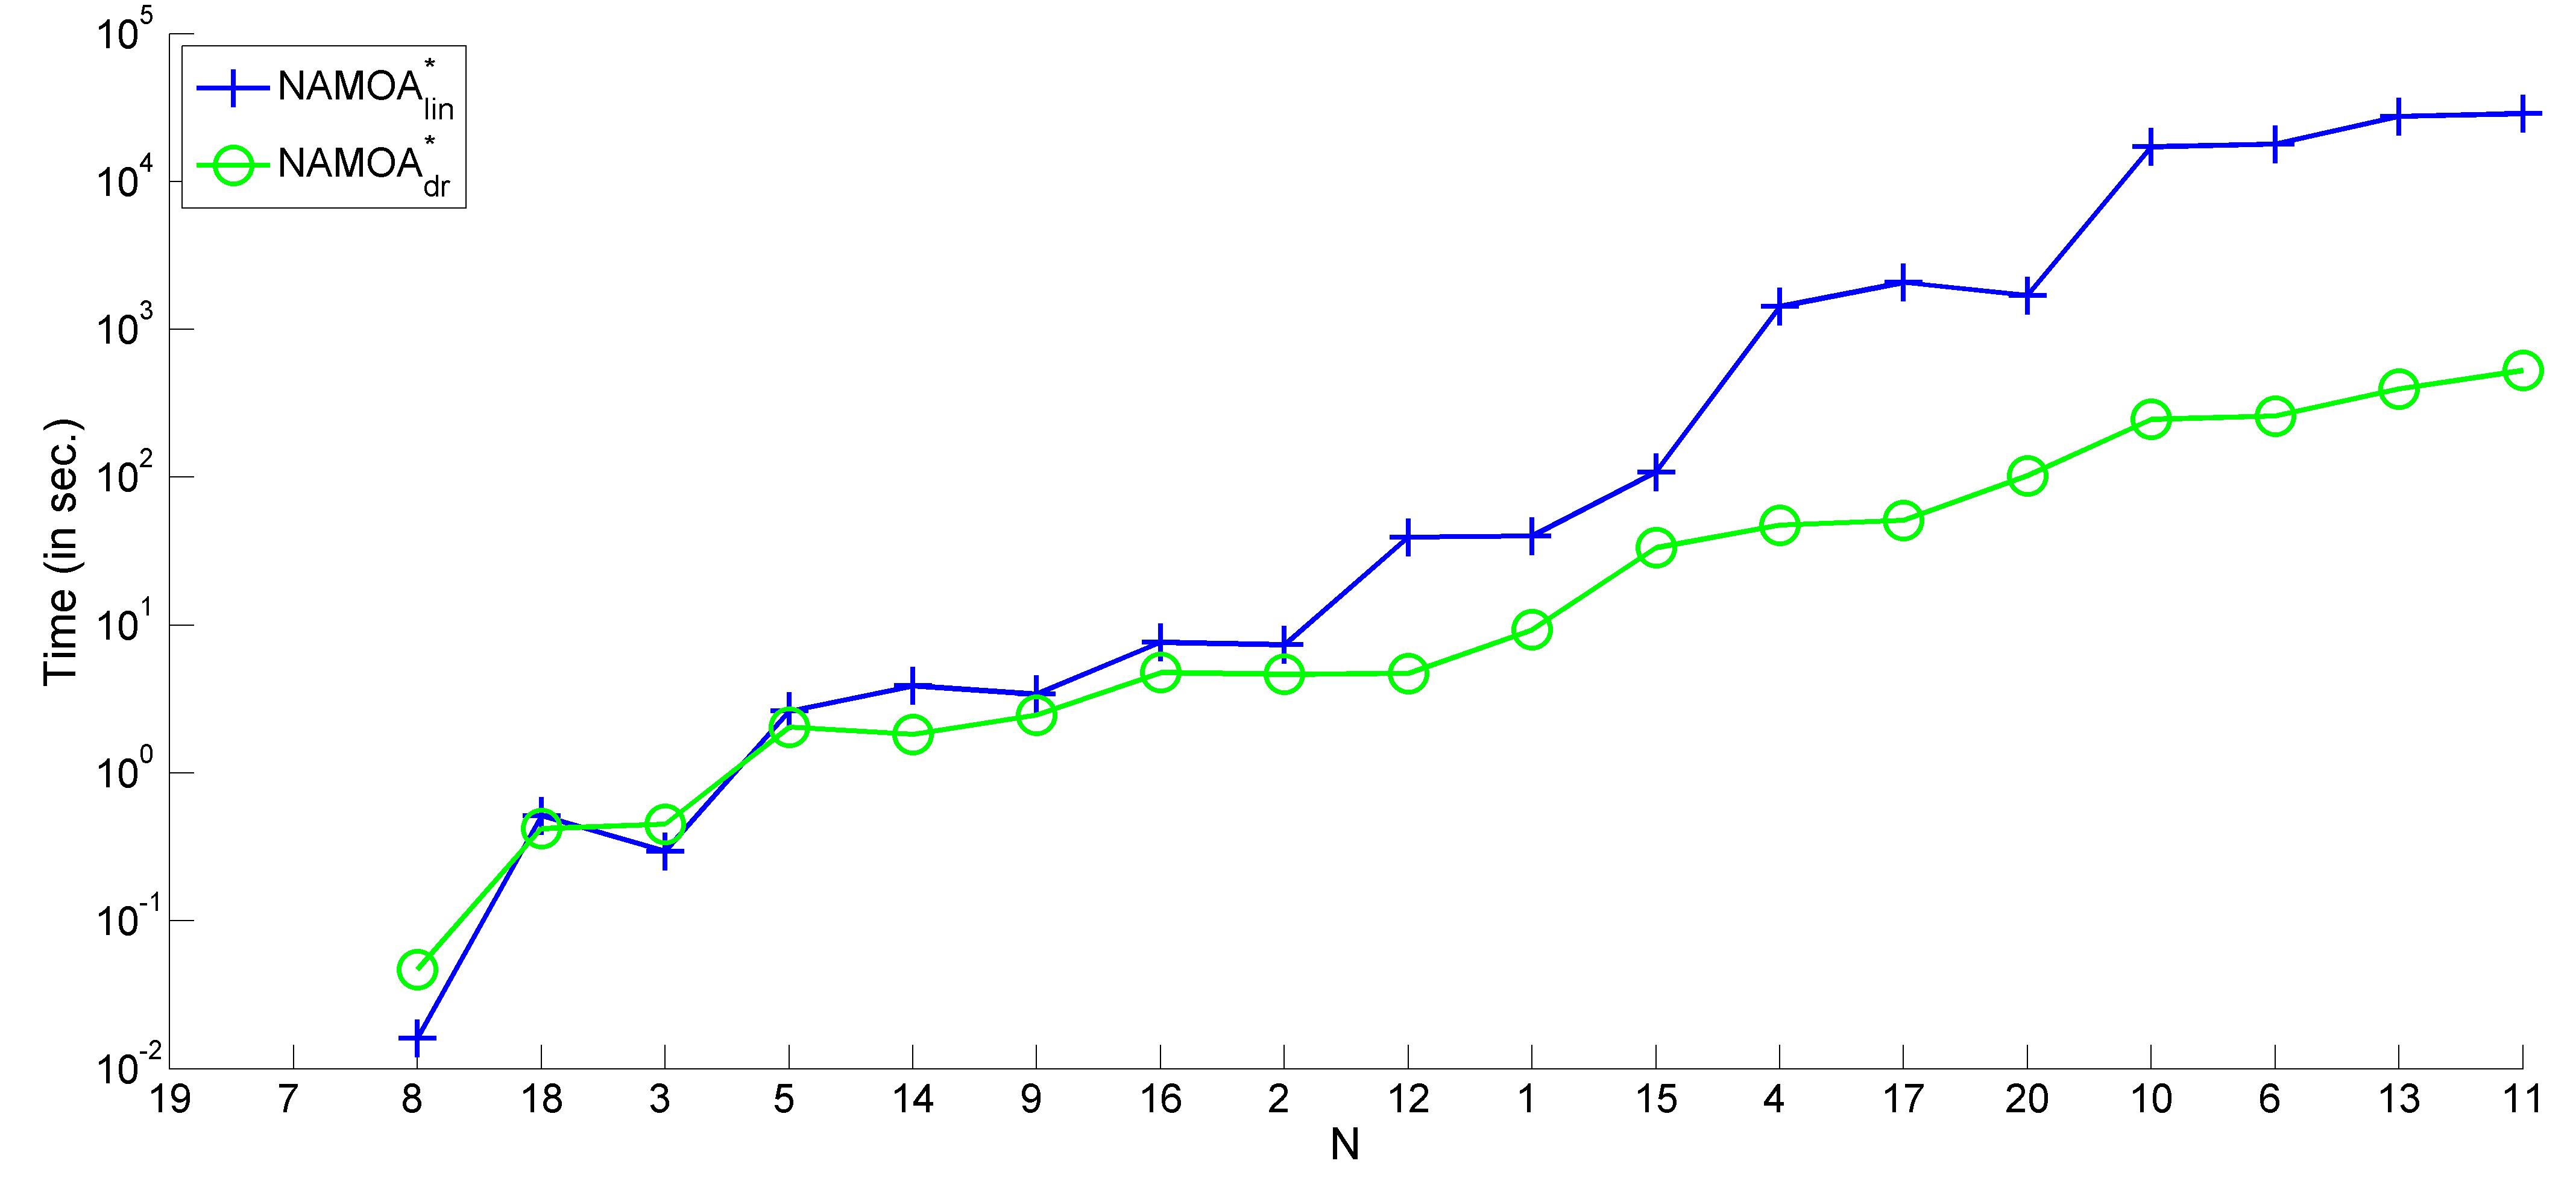
\includegraphics[width=1\textwidth]{Images/Chapter7/exe-times-VTcut}
\caption{Runtimes of \namoalin \ and \namoate \ for the VT$_{cut}$ map problems sorted by the number of labels expanded.}
\label{fig:7-3}
\end{figure}

Finally, Figures \ref{fig:7-4a} and \ref{fig:7-4b} show the percentage of labels filtered, pruned by open, and pruned by closed node labels over the total number of discarded labels by \namoate, for the maps of NY city and Vermont, respectively. The $X$-axis shows problem ids sorted by the number of scanned labels.

\begin{figure}
    \begin{center}
%
      \subfigure[NY city map]{%
            \label{fig:7-4a}
        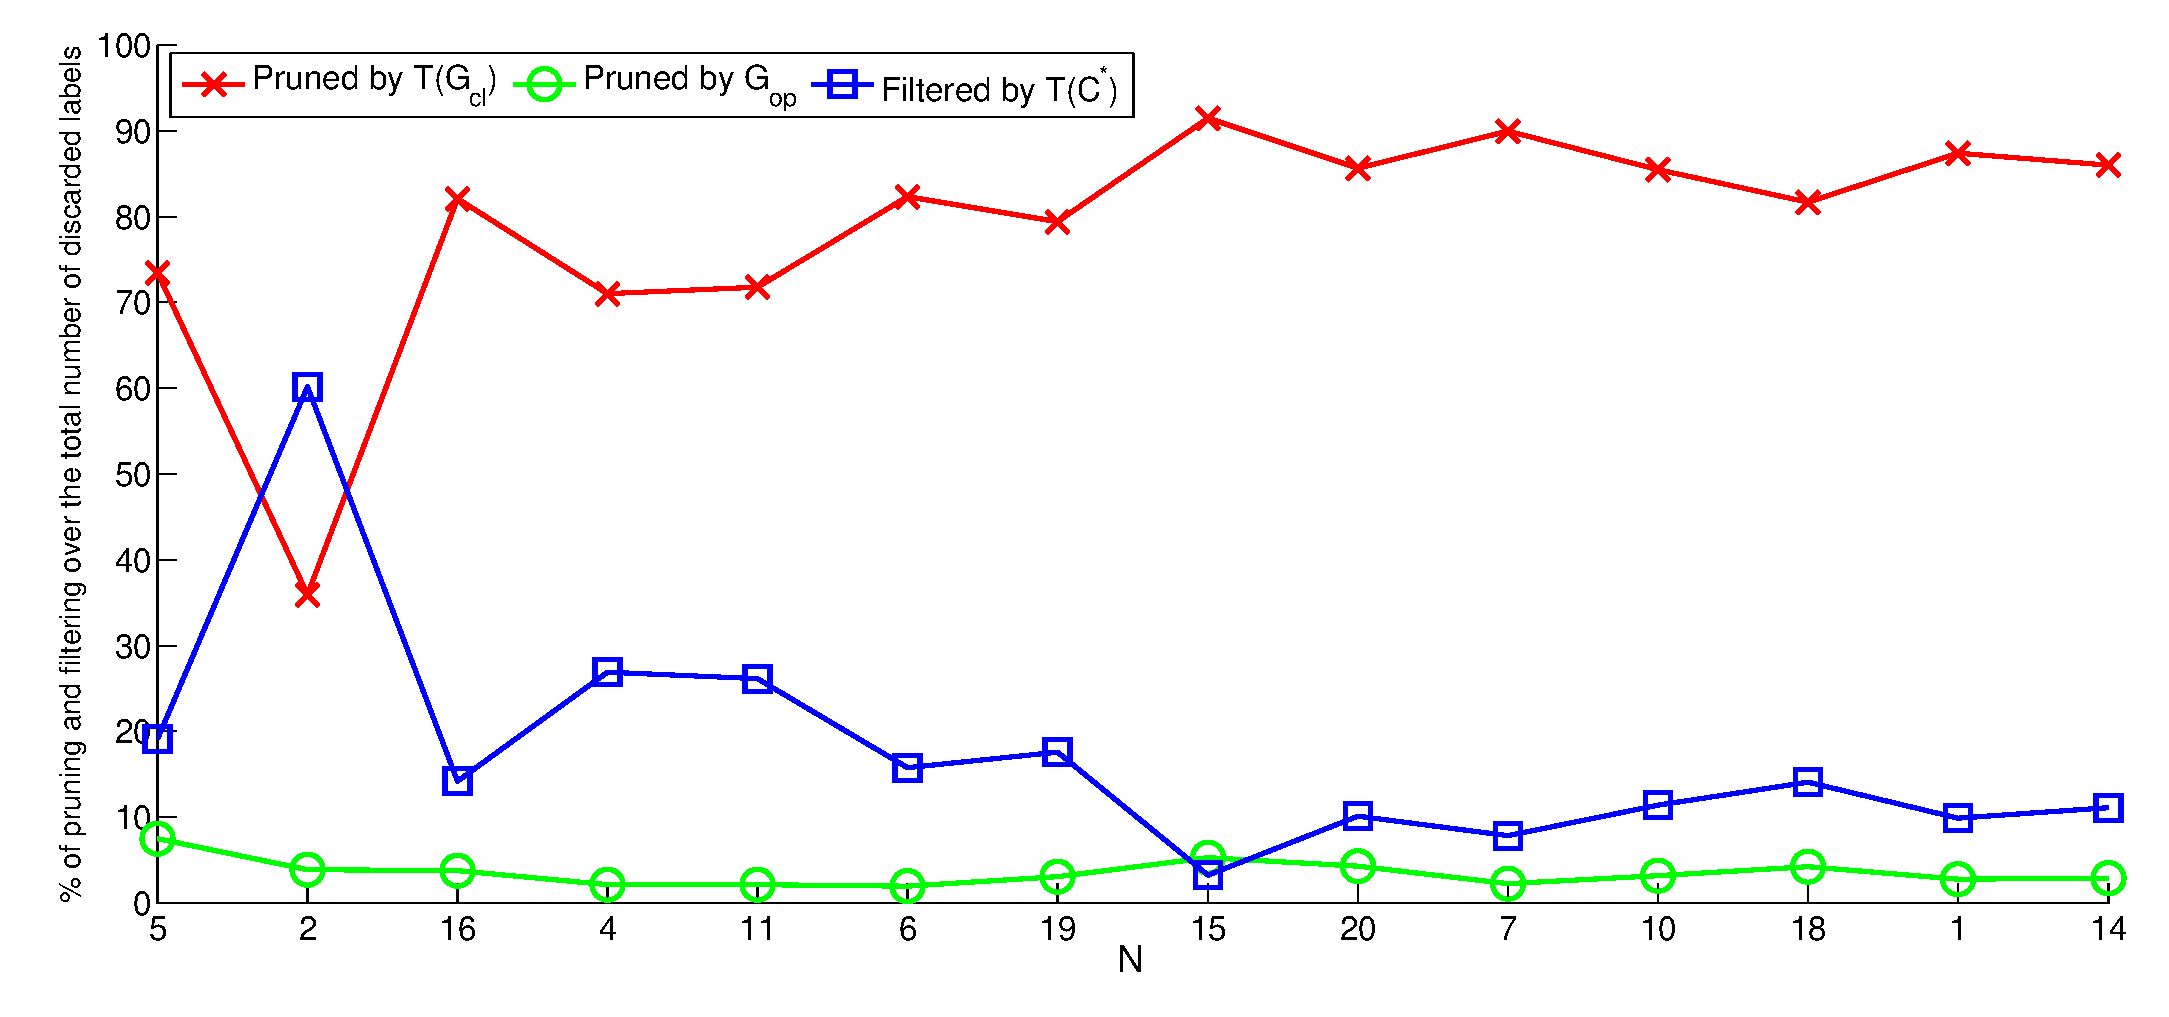
\includegraphics[width=0.95\textwidth]{Images/Chapter7/pruned-filtered-labels-dimacs-perc-NY}
        }\\ %  ------- End of the first row ----------------------%
      \subfigure[Vermont state map]{%
       		\label{fig:7-4b}  
 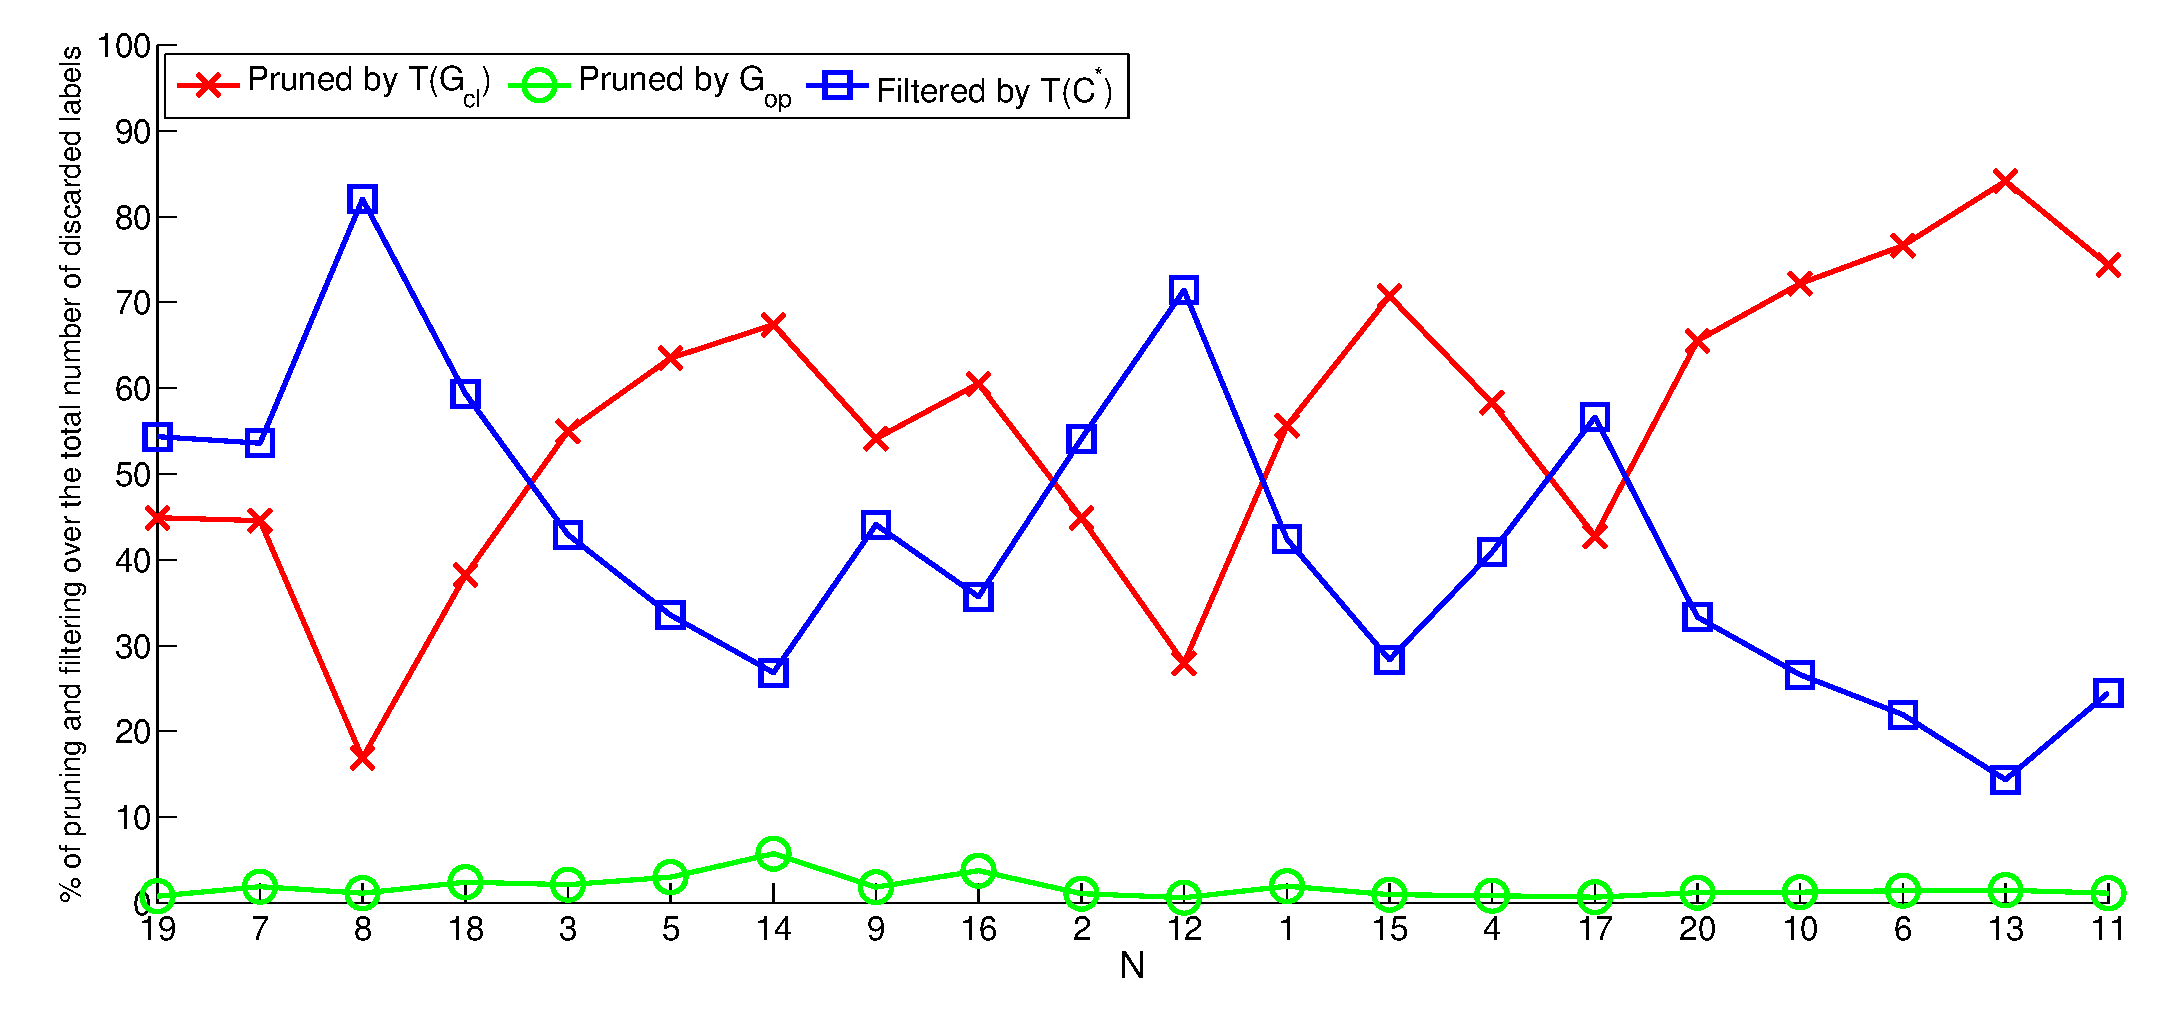
\includegraphics[width=0.95\textwidth]{Images/Chapter7/pruned-filtered-labels-dimacs-perc-VTcut}
        }\\ %  ------- End of the first row ----------------------%
    \end{center}
    \vspace{-0.25in} 
    \caption{%
Percentage of pruned and filtered labels over the total number of discarded labels by \namoate \ per solution depth in road map experiments.  
    }%
    \label{fig:7-4}

\end{figure}

The experiments on the realistic road map problems are much harder than the random grid problems. The largest solvable one (NY\#14) requiring up to 278 million label expansions (the deepest grid problems involved in average 2.5 million label expansions, and 3.3 million in the worst case). Again, \namoate \ clearly outperformed \namoalin, which could only solve problems involving less than 10.1 million label expansions (VT\#11). For such a problem, \namoate \ required only 1.83\% of the time needed by \namoalin. 

On one hand, \namoalin \ was capable of solving within the time limit only 4 problems from the NY set (20\%), while \namoate \ solved 14 (70\%) (see Table \ref{tab:7-13}), and on the other hand, in the test set of VT$_{cut}$ map, which was entirely solved by both algorithms, \namoate \ requires 1.74\% of the time needed by \namoalin (see Table \ref{tab:7-14}). Notice that for the NY map the algorithms were not capable of solving several problem instances in the given 8 hour time limit. These are indicated by symbol ``-'' in the table. Problems \#11 and \#6 were solved by \namoalin \ without time limit in 31 hours and 25 days, respectively.

Except for the simpler problems, cl-pruning was responsible for around 70 to 80\% of the discarded labels (see Figures \ref{fig:7-4a} and \ref{fig:7-4b}). In general, the ratio of filtered labels was larger than those discarded by op-pruning. Once again, this explains the efficiency achieved by t-discarding. Tables \ref{tab:7-12} and \ref{tab:7-13} show dramatic reductions in the sizes of the sets used for cl-pruning and filtering. For the hardest solved instance (NY\#14), the size of $T(\text{C}^*)$ is just $0.32\%$ the size of $\text{C}^*$. For the sets of closed labels, the ratio is $2.26\%$.

\begin{table}
\caption{Summary of $VT_{cut}$ map results.}
\label{tab:7-14}
\begin{center}
\begin{tabular}{ccccccc}
\hline \noalign{\smallskip}
Map & $(\frac{\sum G_{cl}}{\sum T(G_{cl})})$\% & $(\frac{\sum C^*}{\sum T(C^*)})$\% & $C^*$ & $t_{\text{NAMOA}^* \text{lin}}$ & $t_{\text{NAMOA}^* \text{dr}}$ & \% \\
\noalign{\smallskip} \hline 
%NY(2) & 4.56 & 2.25 & 2,164.1 & 2,988.1 & 132.2 & 4.42 \\
VT$_{cut}$ & 3.43 & 2.45 & 3,334.6 & 4,838.4 & 84.6 & 1.74 \\
%DE & 57.76 & 34.61 & 93 & 1.34 & 1.16 & 86.56 \\
\hline
\end{tabular} 
\end{center}
\end{table}

%-------------------------------------------------------------------
\subsection{Summary}
\label{chapEmpiricalAnalysis:subsec:summarydimacsnamoate}
%-------------------------------------------------------------------

The proposed t-discarding procedure proves to be very effective, reducing the time requirements over an order of magnitude over the most efficient search with the standard dominance checks. The new technique effectively extends the size of the three-objective problems that can be practically solved and opens a range of possibilities for multiobjective search algorithms to become more time-efficient. Thus, we then analyze the runtime performance of the application of this technique to the algorithm \lexgo.

%-------------------------------------------------------------------
\section{\texorpdfstring{\lexgote}{LEXGO*dr} \ vs \texorpdfstring{\lexgo}{LEXGO*}}
\label{chapEmpiricalAnalysis:sec:resultsdimacslexgote}
%-------------------------------------------------------------------

This section analyzes the three versions of \lexgo \ already presented, \lexgolex, \lexgolin, and \lexgote. A detailed description of \lexgo \ and \lexgote \ are presented in Sections \ref{chapMultiObjAlg:subsec:lexgo} and \ref{chapMultiObjAlg:subsec:lexgote}, respectively. 

The experiments below analyze the impact of the dimensionality reduction technique over the sets of random road map problems previously used, employing the goals already described in previous sections. The analysis is conducted over the Vermont problems and the NY city problems able to be solved by \lexgolex \ or \lexgolin. Notice that for a problem to be considered solved, all class I and II experiments must be solved within the time limit. The standard versions of \lexgo \ solved four and \lexgote \ six out of the twenty problems considered in the NY city map. 

%-------------------------------------------------------------------
\subsection{Analysis on class I experiments}
\label{chapEmpiricalAnalysis:subsec:analysisdimacslexgotec1}
%-------------------------------------------------------------------

Table \ref{tab:7-15} displays all the runtimes in seconds corresponding to Vermont and NY city problems solved by \lexgote. Table \ref{tab:7-16} summarizes the average execution times of Vermont problems for \lexgolex, \lexgolin, and \lexgote. Finally, Table \ref{tab:7-17} shows the runtimes of \lexgolex, \lexgolin, and \lexgote \ for problems NY\#4 and NY\#16 (runtimes of problems NY\#2 and NY\#5 are not shown since they are too small to be significative). 

In this first class of problems, \lexgote \ has a substantial advantage over both standard versions of \lexgo. \lexgote \ solves the full set of Vermont problems in 1.87\% and 2.01\% of the time needed by \lexgolex \ and \lexgolin \ when $k_1 = 1$, respectively. The time needed by \lexgote \ is 2.21\% and 2.39\%, and 3.91\% and 4.45\% with respect to \lexgolex \ and \lexgolin \ when $k_1 = 0.75$ and $k_1 = 0.5$. Regarding the experiments where the goals cannot be satisfied, the improvement of \lexgote \ is 11.45\% and 23.55\% over \lexgolex \ and \lexgolin \ when $k_1 = 0.25$, respectively, whereas all the runtimes when $k_1 = 0$ are equal to 0.03 seconds. It is also worth noting that the runtime of \lexgote \ when $k_1 = 0.25$ is greater than the runtimes when goals can be satisfied, i.e. when $k_1 = \{1, 0.75, 0.5\}$. This is due to the fact that the t-discarding technique is only applied to \lexgo \ when goals can be satisfied, hence, few problems when $k_1 = 0.25$ can benefit from the dimensionality reduction technique.

Let's turn now our attention to the NY city problems. Regarding problem NY\#4, \lexgote \ is more than twenty times faster than \lexgolex \ and \lexgolin \ when $k_1=\{1, 0.75\}$, sixteen times faster when $k_1=0.5$, and it has a similar performance when goals cannot be satisfied, i.e. when $k_1=\{0.25, 0\}$. 

\begin{table}
\caption{Class I experiments in road maps, runtimes in seconds of \lexgote \ for the experiments over Vermont and NY city maps.}
\label{tab:7-15}
\centering
\begin{tabular}{crrrrrrrr}
\hline \noalign{\smallskip}
& & \multicolumn{4}{c}{\lexgote} \\
\noalign{\smallskip} \cline{3-7} \noalign{\smallskip}
& $n$ & 1 & 0.75 & 0.5 & 0.25 & 0 & \multicolumn{1}{c}{$k_1$}\\
\noalign{\smallskip} 
\cline{1-8} \noalign{\smallskip} 
\parbox[t]{2mm}{\multirow{20}{*}{\rotatebox[origin=c]{90}{Vermont}}} &
1 & 9.68 & 4.71 & 1.35 & 0.45 & <0.01 \\
& 2 & 4.99 & 2.49 & 2.44 & 1.29 & 0.06 \\
& 3 & 0.68 & 0.42 & 0.20 & 0.18 & 0.03 \\
& 4 & 55.58 & 43.72 & 18.42 & 4.10 & 0.03 \\
& 5 & 2.37 & 1.82 & 0.59 & 0.06 & 0.04 \\
& 6 & 291.90 & 278.64 & 175.31 & 32.85 & 0.03 \\
& 7 & <0.01 & <0.01 & <0.01 & <0.01 & <0.01 \\
& 8 & 0.03 & <0.01 & <0.01 & <0.01 & <0.01 \\
& 9 & 3.16 & 2.15 & 1.37 & 0.60 & <0.01 \\
& 10 & 265.2 & 258.7 & 117.81 & 274.95 & 0.10 \\
& 11 & 584.45 & 427.56 & 401.99 & 357.66 & 0.09 \\
& 12 & 5.50 & 1.96 & 0.60 & 0.18 & 0.03 \\
& 13 & 464.60 & 491.77 & 332.82 & 2413.64 & 0.06 \\
& 14 & 2.10 & 1.87 & 0.95 & 0.10 & <0.01 \\
& 15 & 33.36 & 30.60 & 23.35 & 1.32 & 0.09 \\
& 16 & 4.52 & 1.90 & 1.70 & 0.88 & <0.01 \\
& 17 & 61.37 & 43.24 & 14.90 & 9.26 & 0.07 \\
& 18 & 0.37 & 0.24 & 0.32 & 0.07 & <0.01 \\
& 19 & <0.01 & <0.01 & <0.01 & <0.01 & <0.01 \\
& 20 & 108.15 & 80.15 & 53.52 & 43.00 & 0.03 \\
\noalign{\medskip}
\parbox[t]{2mm}{\multirow{6}{*}{\rotatebox[origin=c]{90}{NY city}}} &
2 & 0.87 & 0.65 & 0.28 & 0.01 & <0.01 \\
& 4 & 201.64 & 198.18 & 176.04 & 63.94 & 0.03 \\
& 5 & <0.01 & <0.01 & <0.01 & <0.01 & <0.01  \\
& 11 & 1,753.57 & 1,668.50 & 1,366.86 & 3,664.96 & 0.07 \\
& 16 & 118.63 & 116.22 & 62.97 & 0.96 & 0.01 \\
& 19 & 10,873.42 & 10,960.56 & 10,005.21 & 1,506.29 & 0.45 \\
\hline
\end{tabular}
\end{table}

\begin{table}
\caption{Class I experiments in road maps, summary of Vermont problems runtimes in seconds of \lexgolex, \lexgolin \ and \lexgote.}
\label{tab:7-16}
\centering
\begin{tabular}{rrrrrrrr}
\hline \noalign{\smallskip}
 & 1 & 0.75 & 0.5 & 0.25 & 0 & \multicolumn{1}{c}{$k_1$}\\
\noalign{\smallskip} 
\cline{2-6} \noalign{\smallskip} 
\lexgolex & 5,068.00 & 3,769.51 & 1,467.00 & 177.33 & 0.03 \\
\lexgolin & 4,716.90 & 3,497.26 & 1,287.37 & 205.39 & 0.03 \\
\lexgote & 94.90 &	83.59 & 57.38 & 157.02 & 0.03 \\
\hline
\end{tabular}
\end{table}


\begin{table}
\caption{Class I experiments in road maps, runtimes of \lexgolex, \lexgolin, and \lexgote \ for two NY city problems.}
\label{tab:7-17}
\centering
\scalebox{0.92}{
\begin{tabular}{lrrrrrr}
\hline %\noalign{\smallskip}
Problem & \multicolumn{3}{c} 4 & \multicolumn{3}{c}{16} \\
%\noalign{\smallskip} 
\hline
Algorithm & \lexgolex & \lexgolin & \lexgote & \lexgolex & \lexgolin & \lexgote \\
$(k_1=1)$    & 4,845.19 & 4,379.98 & 201.64 & 458.64 & 508.23 & 118.63 \\ 
$(k_1=0.75)$ & 4,038.80 & 4,184.89 & 198.18 & 234.34 & 370.87 & 116.22 \\ 
$(k_1=0.5)$  & 2,829.04   & 3,407.90 & 176.04  & 63.26  & 78.54 & 62.97\\ 
$(k_1=0.25)$ & 74.89   &  172.52 & 63.94 & 1.03    & 1.01 & 0.96 \\ 
$(k_1=0)$    & 0.01   &   0.03 & 0.03 & 0.01  & 0.01 & 0.01\\ 
\hline
\end{tabular}
}
\end{table}

%-------------------------------------------------------------------
\subsection{Analysis on class II experiments}
\label{chapEmpiricalAnalysis:subsec:analysisdimacslexgotec2}
%-------------------------------------------------------------------

Regarding the class II experiments, Table \ref{tab:7-18} displays all the runtimes in seconds corresponding to Vermont and NY city problems solved by \lexgote. The average runtimes of Vermont problems for \lexgolex, \lexgolin, and \lexgote \ are summarized in Table \ref{tab:7-19}. 

In these experiments, \lexgote \ also outperforms \lexgolex \ and \lexgolin. The relative advantage of \lexgote \ over \lexgolex \ and \lexgolin \ grows when the number of goal-optimal solution vectors is greater, as well as with the size of the problem. Thus, the time needed by \lexgote \ to solve the full set of Vermont problems is 41.87\% of the time needed by \lexgolex \ when $k_1 = 0.5$ and $k_2 = 0.125$. This comparative advantage grows to its maximum when $k_1 = k_2 = 0.75$, where \lexgote \ runtime is 2.21\% of \lexgolex \ runtime, i.e. \lexgote \ is more than 45 times faster than \lexgolex.

Table \ref{tab:7-20} shows a comparative of \lexgolex, \lexgolin, and \lexgote \ runtimes for problems NY\#4 and NY\#16. Problem NY\#16 does not show an apparent improvement when using \lexgote \ in many cases, since those cases cannot satisfy the provided goals. 

\begin{table}
\caption{Class II experiments in road maps, runtimes in seconds of \lexgote \ for the experiments over Vermont and NY city maps.}
\label{tab:7-18}
\centering
\scalebox{.78}{
\begin{tabular}{crrrrrrrrrrr}
\hline \noalign{\smallskip}
& & & \multicolumn{8}{c}{\lexgote} & \\
\noalign{\smallskip} \cline{3-10}
& & \multicolumn{4}{c|}{0.75} & \multicolumn{4}{c}{0.5} & \multicolumn{1}{c}{$k_1$}\\
& $n$  & 0.75 & 0.5625 & 0.375 & \multicolumn{1}{c|}{0.1875} & 0.5 & 0.375 & 0.25 & 0.125 & \multicolumn{1}{c}{$k_2$}\\
\noalign{\smallskip} 
\cline{1-11} \noalign{\smallskip} 
\parbox[t]{2mm}{\multirow{20}{*}{\rotatebox[origin=c]{90}{Vermont}}} &
1 & 4.71 & 4.71 & 6.32 & 13.90 & 1.36 & 1.42 & 1.78 & 2.20 \\ 
& 2 & 2.50 & 3.01 & 2.61 & 2.28 & 2.45 & 2.06 & 1.90 & 1.17 \\ 
& 3 & 0.42 & 0.64 & 0.38 & 0.20 & 0.20 & 0.20 & 0.13 & 0.11 \\ 
& 4 & 43.73 & 46.94 & 31.79 & 22.11 & 18.42 & 8.66 & 2.98 & 5.18 \\ 
& 5 & 1.83 & 1.47 & 0.91 & 0.70 & 0.59 & 0.30 & 0.34 & 0.53 \\ 
& 6 & 278.65 & 266.84 & 184.47 & 58.47 & 175.31 & 211.48 & 93.07 & 281.11 \\ 
& 7 & <0.01 & <0.01 & <0.01 & <0.01 & <0.01 & <0.01 & <0.01 & <0.01 \\ 
& 8 & <0.01 & <0.01 & <0.01 & <0.01 & <0.01 & <0.01 & <0.01 & <0.01 \\ 
& 9 & 2.15 & 1.92 & 1.56 & 1.00 & 1.37 & 0.91 & 0.78 & 0.61 \\ 
& 10 & 258.79 & 200.35 & 134.57 & 26.68 & 117.81 & 81.26 & 57.49 & 146.35 \\ 
& 11 & 427.57 & 418.82 & 394.06 & 264.59 & 402.00 & 395.54 & 313.09 & 209.03 \\ 
& 12 & 1.97 & 1.92 & 1.78 & 0.90 & 0.67 & 0.45 & 0.64 & 0.45 \\ 
& 13 & 491.78 & 450.97 & 438.63 & 144.61 & 332.83 & 304.70 & 189.07 & 17.80 \\ 
& 14 & 1.87 & 1.53 & 1.00 & 0.31 & 0.95 & 0.47 & 0.08 & 0.08 \\ 
& 15 & 30.61 & 28.50 & 24.96 & 26.46 & 23.35 & 22.56 & 22.51 & 15.85 \\ 
& 16 & 1.95 & 2.12 & 2.65 & 2.14 & 1.70 & 1.73 & 1.54 & 1.79 \\ 
& 17 & 43.24 & 43.51 & 35.51 & 25.83 & 14.93 & 10.09 & 1.42 & 1.64 \\ 
& 18 & 0.25 & 0.23 & 0.22 & 0.39 & 0.33 & 0.17 & 0.17 & 0.17 \\ 
& 19 & <0.01 & <0.01 & <0.01 & <0.01 & <0.01 & <0.01 & <0.01 & <0.01 \\ 
& 20 & 80.15 & 92.57 & 84.66 & 97.33 & 53.52 & 36.50 & 31.65 & 38.94 \\ 
\noalign{\medskip}
\parbox[t]{2mm}{\multirow{6}{*}{\rotatebox[origin=c]{90}{NY city}}} &
2 & 0.65 & 0.60 & 0.42 & 0.15 & 0.28 & 0.23 & 0.25 & 0.25 \\
& 4 & 198.18 & 220.77 & 225.99 & 128.49 & 176.04 & 177.32 & 170.47 & 35.67 \\
& 5 & <0.01 & - & - & - & - & - & - & - \\
& 11 & 1,668.50 & 1,617.41 & 2,653.90 & 2,852.52 & 1,366.86 & 1,860.42 & 2,727.67 & 4,532.50 \\
& 16 & 116.22 & 86.22 & 31.18 & 12.69 & 62.97 & 77.39 & 86.87 & 84.35 \\
& 19 & 10,960.56 & 15,407.65 & 20,771.40 & 5,270.44 & 10,005.21 & 12,456.02 & 5,141.12 & 4,519.28 \\
\hline
\end{tabular}
}
\end{table} 

\begin{table}
\caption{Class II experiments in road maps, runtimes in seconds of \lexgote \ for the experiments over Vermont and NY city maps.}
\label{tab:7-19}
\centering
\scalebox{.85}{
\begin{tabular}{rrrrrrrrrr}
\hline \noalign{\smallskip}
\multicolumn{1}{c}{} & \multicolumn{4}{c|}{0.75} & \multicolumn{4}{c}{0.5} & \multicolumn{1}{c}{$k_1$}\\
 & 0.75 & 0.5625 & 0.375 & \multicolumn{1}{c|}{0.1875} & 0.5 & 0.375 & 0.25 & 0.125 & \multicolumn{1}{c}{$k_2$}\\
\noalign{\smallskip} 
\cline{2-9} \noalign{\smallskip}
\lexgolex & 3,769.51 & 3,092.73 & 1,729.26 & 371.33 & 1,467.00 & 980.69 & 479.92 & 86.32 \\
\lexgolin & 3,497.26 & 2,782.82 & 1,781.04 & 424.25 & 1,287.37 & 977.48 & 499.61 & 109.20 \\
\lexgote & 83.59 & 78.30 & 67.31 & 34.40 & 57.39 & 53.93 & 35.93 & 36.15 \\
\hline
\end{tabular}
}
\end{table} 

\begin{table}
\caption{Class II experiments in road maps, runtimes in seconds of \lexgolex, \lexgolin, and \lexgote \ for two NY city problems.}
\label{tab:7-20}
\centering
\scalebox{0.9}{
\begin{tabular}{lrrrrrr}
\hline 
%\noalign{\smallskip}
Problem & \multicolumn{3}{c} 4 & \multicolumn{3}{c}{16} \\
%\noalign{\smallskip} 
\hline
Algorithm & \lexgolex & \lexgolin & \lexgote & \lexgolex & \lexgolin & \lexgote \\
$(0.75, \ 0.75)$ & 4,038.8 & 4,184.9 & 198.1 & 234.3 & 370.8 & 116.2 \\
$(0.75, \ 0.5625)$ & 4,060.7 & 4,229.3 & 220.7 & 121.9 & 219.9 & 86.2\\
$(0.75, \ 0.375)$ & 2,622.8 & 4,222.0 & 226.0 & 33.1 & 55.9 & 31.1\\
$(0.75, \ 0.1875)$ & 267.1 & 762.3 & 128.5 & 12.6 & 15.1 & 12.7\\
\noalign{\smallskip}
$(0.5. \ 0.5)$ & 2,829.0 & 3,407.9 & 176.0 & 63.2 & 78.5 & 62.9\\
$(0.5. \ 0.375)$ & 1,894.2 & 2,819.4 & 177.3 & 77.8 & 88.9 & 77.3\\
$(0.5. \ 0.25)$ & 627.1 & 1,757.5 & 170.5 & 84.3 & 92.9 & 86.8\\
$(0.5. \ 0.125)$ & 41.0 & 148.0 & 35.6 & 85.6 & 96.0 & 84.3\\  
\hline
\end{tabular}
}
\end{table}

%-------------------------------------------------------------------
\subsection{Summary}
\label{chapEmpiricalAnalysis:subsec:summarydimacslexgote}
%-------------------------------------------------------------------

In a similar manner as \lexgote \ outperforms \lexgo \ in random grids, the results do not change for road map problems. A greater speed-up can be observed in these experiments. When a large number of goal-optimal solution vectors from the Pareto frontier satisfy the goals, the t-discarding method is applied to a greater extent to \lexgote \ and speeds up the performance to up to 50 times faster than any previous version of \lexgo. Since this advantage grows with difficulty, the obtained results point out that \lexgote \ must be chosen over \lexgo \ in problems with a certain level of difficulty and satisfiable goals, although when goals cannot be satisfied \lexgote \ does only contribute with a slight advantage. 

%-------------------------------------------------------------------
\section{\texorpdfstring{\lexgote}{LEXGO*dr} \ vs \texorpdfstring{\namoate}{NAMOA*dr}}
\label{chapEmpiricalAnalysis:sec:resultsdimacste}
%-------------------------------------------------------------------

This section considers \namoate \ and \lexgote, versions of \namoa \ and \lexgo \ that employ the t-discarding technique described in Section \ref{chapMultiObjAlg:sec:Time-efficient-MSalg}. Since t-discarding can only be applied to \lexgo \ when goals can be satisfied, the question of its comparative performance to \namoate \ also arises for the road map problems. 

\namoate \ has been empirically proved to be more efficient than \namoa. In the same manner, \lexgote \ outperforms \lexgo. \namoate \ obtains a greater ratio of improvement over the standard versions of \namoa \ than \lexgote \ achieves over their counterparts of \lexgo. Thus, a final comparative analysis for random map problems between \namoate \ and \lexgote \ is presented in this section.  

The experiments are applied to the road map problems previously used. The goals employed to define the set of goal-optimal solution vectors are defined analogously as in Section \ref{chapEmpiricalAnalysis:sec:grids}. The analysis is conducted over the Vermont problems and the NY city problems able to be solved by \lexgote \ and \namoate, which were six and fourteen out of twenty, respectively.

%-------------------------------------------------------------------
\subsection{Analysis on class I experiments}
\label{chapEmpiricalAnalysis:subsec:analysisdimacstec1}
%-------------------------------------------------------------------

In Table \ref{tab:7-21} the results of \namoate \ and \lexgote \ are presented. Cases where \lexgote \ runtimes are faster than runtimes of \namoate \ are highlighted in bold. The average runtimes of the full set of Vermont map experiments are shown in Table \ref{tab:7-22}.

An expected overhead in \lexgote \ over \namoate \ is found when $k_1 = 1$. In this case, the overhead corresponding to the extra deviation pruning and filtering efforts represents 12.08\% of the runtime of \namoate. \lexgote \ shows a very similar runtime in average when $k_1 = 0.75$, only 1.26\% faster. When $k_1 = 0.5$, \lexgote \ clearly outperforms \namoate, being 32.22\% more efficient in runtime. As always, when the goals are located in the ideal point ($k_1 = 0$), \lexgote, with an average runtime of three hundredths of a second, outperforms \namoate.

A particular case of \lexgote \ can be observed in $k_1 = 0.25$ case. Problem VT\#13 is solved by \lexgote \ more than six times slower than by \namoate, and problem NY\#11 two and a half times slower. In order to understand this behavior we measured the percentage of times that a pruning operation is conducted in a time-efficient manner with respect to the total of pruning operations. We call this quotient $\eth$. Thus, $\eth_{13VT} = 0.4698$ and $\eth_{11NY} = 0.6938$ while other problems of similar difficulty, VT\#11 for example, present a much higher value ($\eth_{11} = 0.9531$). In other words, problem VT\#13 cannot use the Pareto pruning (dr) as often as the rest of the problems, in this case only 46.98\% of the times, and hence, its runtime is much higher than the average.

\begin{table}
\caption{Class I experiments in road maps, runtimes in seconds of \namoate \ and \lexgote \ for the experiments over Vermont and NY city maps.}
\label{tab:7-21}
\centering
\begin{tabular}{crrrrrrrrr}
\hline \noalign{\smallskip}
& & & \multicolumn{4}{c}{\lexgote} \\
\noalign{\smallskip} \cline{4-8} \noalign{\smallskip}
& $n$ & \namoate & 1 & 0.75 & 0.5 & 0.25 & 0 & \multicolumn{1}{c}{$k_1$}\\
\noalign{\smallskip} 
\cline{1-8} \noalign{\smallskip} 
\parbox[t]{2mm}{\multirow{20}{*}{\rotatebox[origin=c]{90}{Vermont}}} &
1 & \textbf{9.29} & 9.68 & \textbf{4.71} & \textbf{1.35} & \textbf{0.45} & \textbf{<0.01} \\
& 2 & \textbf{4.64} & 4.99 & \textbf{2.49} & \textbf{2.44} & \textbf{1.29} & \textbf{0.06} \\
& 3 & \textbf{0.45} & 0.68 & \textbf{0.42} & \textbf{0.20} & \textbf{0.18} & \textbf{0.03} \\
& 4 & \textbf{47.53} & 55.58 & \textbf{43.72} & \textbf{18.42} & \textbf{4.10} & \textbf{0.03} \\
& 5 & \textbf{2.04} & 2.37 & \textbf{1.82} & \textbf{0.59} & \textbf{0.06} & \textbf{0.04} \\
& 6 & \textbf{259.05} & 291.90 & 278.64 & \textbf{175.31} & \textbf{32.85} & \textbf{0.03} \\
& 7 & \textbf{<0.01} & \textbf{<0.01} & \textbf{<0.01} & \textbf{<0.01} & \textbf{<0.01} & \textbf{<0.01} \\
& 8 & \textbf{<0.01} & \textbf{<0.01} & \textbf{<0.01} & \textbf{<0.01} & \textbf{<0.01} & \textbf{<0.01} \\
& 9 & \textbf{2.46} & 3.16 & \textbf{2.15} & \textbf{1.37} & \textbf{0.60} & \textbf{<0.01} \\
& 10 & \textbf{246.09} & 265.20 & 258.70 & \textbf{117.81} & 274.95 & \textbf{0.10} \\
& 11 & \textbf{527.56} & 584.45 & \textbf{427.56} & \textbf{401.99} & \textbf{357.66} & \textbf{0.09} \\
& 12 & \textbf{4.71} & 5.50 & \textbf{1.96} & \textbf{0.60} & \textbf{0.18} & \textbf{0.03} \\
& 13 & \textbf{395.24} & 464.60 & 491.77 & \textbf{332.82} & 2,413.64 & \textbf{0.06} \\
& 14 & \textbf{1.82} & 2.10 & 1.87 & \textbf{0.95} & \textbf{0.10} & \textbf{<0.01} \\
& 15 & \textbf{33.35} & 33.36 & \textbf{30.60} & \textbf{23.35} & \textbf{1.32} & \textbf{0.09} \\
& 16 & \textbf{4.77} & \textbf{4.52} & \textbf{1.90} & \textbf{1.70} & \textbf{0.88} & \textbf{<0.01} \\
& 17 & \textbf{51.26} & 61.37 & \textbf{43.24} & \textbf{14.90} & \textbf{9.26} & \textbf{0.07} \\
& 18 & \textbf{0.42} & \textbf{0.37} & \textbf{0.24} & \textbf{0.32} & \textbf{0.07} & \textbf{<0.01} \\
& 19 & \textbf{<0.01} & \textbf{<0.01} & \textbf{<0.01} & \textbf{<0.01} & \textbf{<0.01} & \textbf{<0.01} \\
& 20 & \textbf{102.57} & 108.15 & \textbf{80.15} & \textbf{53.52} & \textbf{43.00} & \textbf{0.03} \\
\noalign{\medskip}
\parbox[t]{2mm}{\multirow{6}{*}{\rotatebox[origin=c]{90}{NY city}}} &
2 & \textbf{0.71} & 0.87 & \textbf{0.65} & \textbf{0.28} & \textbf{0.01} & \textbf{<0.01} \\
& 4 & \textbf{149.30} & 201.64 & 198.18 & 176.04 & \textbf{63.94} & \textbf{0.03} \\
& 5 & \textbf{<0.01} & \textbf{<0.01} & \textbf{<0.01} & \textbf{<0.01} & \textbf{<0.01} & \textbf{<0.01} \\
& 11 & \textbf{1,452.58} & 1,753.57 & 1,668.50 & \textbf{1,366.86} & 3,664.96 & \textbf{0.07} \\
& 16 & \textbf{106.89} & 118.63 & 116.22 & \textbf{62.97} & \textbf{0.96} & \textbf{0.01} \\
& 19 & \textbf{8,355.32} & 10,873.42 & 10,960.56 & 10,005.21 & \textbf{1,506.29} & \textbf{0.45} \\
\hline
\end{tabular}
\end{table}

\begin{table}
\caption{Class I experiments in road maps, average runtimes in seconds of \namoate \ and \lexgote \ for the set of Vermont map experiments.}
\label{tab:7-22}
\centering
\begin{tabular}{rrrrrrr}
\hline \noalign{\smallskip}
 & \multicolumn{5}{c}{\lexgote} \\
\noalign{\smallskip} \cline{2-6} \noalign{\smallskip}
\namoate & 1 & 0.75 & 0.5 & 0.25 & 0 & \multicolumn{1}{c}{$k_1$}\\
\noalign{\smallskip} 
\cline{1-6} \noalign{\smallskip} 
84.66 & 94.89 & 83.59 & 57.38 & 157.02 & 0.03 \\
\hline
\end{tabular}
\end{table}

%-------------------------------------------------------------------
\subsection{Analysis on class II experiments}
\label{chapEmpiricalAnalysis:subsec:analysisdimacstec2}
%-------------------------------------------------------------------

Regarding the second class of problems, unlike \lexgolex \ and \lexgolin \ with their \namoa \ counterparts, when applying the t-discarding technique to \lexgo \ and \namoa , \lexgote \ does not perform always faster than \namoate \ when $k_2$ values become stricter, in fact, the runtimes eventually increase notably although the number of label expansions decrease. This is due to the t-discarding method only applies to \lexgote \ when goals can be satisfied.

Table \ref{tab:7-23} displays the runtimes in seconds of \namoate \ and \lexgote \ for the Vermont and New York city maps experiments. Table \ref{tab:7-24} displays a summary of the average runtime of the full set of Vermont map experiments. On one hand, \lexgote \ outperforms in average \namoate \ in the Vermont map experiments, on the other hand, for the two most difficult problems solved by both algorithms, NY\#11 and NY\#19, \lexgote \ only runs faster than \namoate \ in three of the sixteen cases available. 

\begin{table}
\caption{Class II experiments in road maps, runtimes in seconds of \namoate \ and \lexgote \ for the experiments over Vermont and NY city maps.}
\label{tab:7-23}
\centering
\scalebox{.69}{
\begin{tabular}{crrrrrrrrrrrr}
\hline \noalign{\smallskip}
& & & \multicolumn{4}{c}{\lexgote} \\
\noalign{\smallskip} \cline{4-11} \noalign{\smallskip}
& & & \multicolumn{4}{c|}{0.75} & \multicolumn{4}{c}{0.5} & \multicolumn{1}{c}{$k_1$}\\
& $n$ & \namoate & 0.75 & 0.5625 & 0.375 & \multicolumn{1}{c|}{0.1875} & 0.5 & 0.375 & 0.25 & 0.125 & \multicolumn{1}{c}{$k_2$}\\
\noalign{\smallskip} 
\hline \noalign{\smallskip} 
\parbox[t]{2mm}{\multirow{20}{*}{\rotatebox[origin=c]{90}{Vermont}}} &
1 & \textbf{9.29} & \textbf{4.71} & \textbf{4.71} & \textbf{6.31} & 13.90 & \textbf{1.35} & \textbf{1.42} & \textbf{1.77} & \textbf{2.20}\\
& 2 & \textbf{4.64} & \textbf{2.49} & \textbf{3.01} & \textbf{2.60} & \textbf{2.27} & \textbf{2.44} & \textbf{2.05} & \textbf{1.90} & \textbf{1.17} \\
& 3 & \textbf{0.45} & \textbf{0.42} & 0.64 & \textbf{0.37} & \textbf{0.20} & \textbf{0.20} & \textbf{0.20} & \textbf{0.12} & \textbf{0.10} \\
& 4 & \textbf{47.53} & \textbf{43.72} & \textbf{46.94} & \textbf{31.79} & \textbf{22.10} &\textbf{18.42} & \textbf{8.65} & \textbf{2.97} & \textbf{5.17} \\
& 5 & \textbf{2.04} & \textbf{1.82} & \textbf{1.46} & \textbf{0.90} & \textbf{0.70} & \textbf{0.59} & \textbf{0.29} & \textbf{0.34} & \textbf{0.53} \\
& 6 & \textbf{259.05} & 278.64 & 266.84 & \textbf{184.47} & \textbf{58.46} & \textbf{175.31} & \textbf{211.47} & \textbf{93.07} & 281.11 \\
& 7 & \textbf{<0.01} & \textbf{<0.01} & \textbf{<0.01} & \textbf{<0.01} & \textbf{<0.01} & \textbf{<0.01} & \textbf{<0.01} & \textbf{<0.01} & \textbf{<0.01}\\
& 8 & \textbf{<0.01} & \textbf{<0.01} & \textbf{<0.01} & \textbf{<0.01} & \textbf{<0.01} & \textbf{<0.01} & \textbf{<0.01} & \textbf{<0.01} & \textbf{<0.01}\\
& 9 & \textbf{2.46} & \textbf{2.15} & \textbf{1.91} & \textbf{1.56} & \textbf{0.99} & \textbf{1.37} & \textbf{0.90} & \textbf{0.78} & \textbf{0.60} \\
& 10 & \textbf{246.09} & 258.70 & \textbf{200.35} & \textbf{134.56} & \textbf{26.67} & \textbf{117.81} & \textbf{81.26} & \textbf{57.48} & \textbf{146.34}  \\
& 11 & \textbf{527.56} & \textbf{427.56} & \textbf{418.81} & \textbf{394.05} & \textbf{264.59} & \textbf{401.99} & \textbf{395.54} & \textbf{313.09} & \textbf{209.02} \\
& 12 & \textbf{4.71} & \textbf{1.96} & \textbf{1.91} & \textbf{1.77} & \textbf{0.90} & \textbf{0.60} & \textbf{0.45} & \textbf{0.64} & \textbf{0.45} \\
& 13 & \textbf{395.24} & 491.77 & 450.96 & 438.62 & \textbf{144.61} & \textbf{332.82} & \textbf{304.70} & \textbf{189.07} & \textbf{17.80} \\
& 14 & \textbf{1.82} & 1.87 & \textbf{1.52} & \textbf{0.99} & \textbf{0.31} & \textbf{0.95} & \textbf{0.46} & \textbf{0.07} & \textbf{0.07} \\
& 15 & \textbf{33.35} & \textbf{30.60} & \textbf{28.50} & \textbf{24.96} & \textbf{26.45} & \textbf{23.35} & \textbf{22.55} & \textbf{22.51} & \textbf{15.84} \\
& 16 & \textbf{4.77} & \textbf{1.90} & \textbf{2.12} & \textbf{2.65} & \textbf{2.13} & \textbf{1.70} & \textbf{1.73} & \textbf{1.54} & \textbf{1.79} \\
& 17 & \textbf{51.26} & \textbf{43.24}  & \textbf{43.50} & \textbf{35.50} & \textbf{25.83} & \textbf{14.90} & \textbf{10.09} & \textbf{1.41} & \textbf{1.63} \\
& 18 & \textbf{0.42} & \textbf{0.24} & \textbf{0.23} & \textbf{0.21} & \textbf{0.39} & \textbf{0.32} & \textbf{0.17} & \textbf{0.17} & \textbf{0.17} \\
& 19 & \textbf{<0.01} & \textbf{<0.01} & \textbf{<0.01} & \textbf{<0.01} & \textbf{<0.01} & \textbf{<0.01} & \textbf{<0.01} & \textbf{<0.01} & \textbf{<0.01}\\
& 20 & \textbf{102.57} & \textbf{80.15} & \textbf{92.57} & \textbf{84.66} & \textbf{97.32} & \textbf{53.52} & \textbf{36.50} & \textbf{31.65} & \textbf{38.93} \\
\noalign{\medskip}
\parbox[t]{2mm}{\multirow{6}{*}{\rotatebox[origin=c]{90}{NY city}}} &
2 & \textbf{0.71} & \textbf{0.65} & \textbf{0.60} & \textbf{0.42} & \textbf{0.15} & \textbf{0.28} & \textbf{0.23} & \textbf{0.24} & \textbf{0.25} & \\
& 4 & \textbf{149.30} & 198.18 & 220.77 & 225.99 & \textbf{128.49} & 176.04 & 177.32 & 170.47 & \textbf{35.67} \\
& 5 & \textbf{<0.01} & \textbf{<0.01} & \textbf{<0.01} & \textbf{<0.01} & \textbf{<0.01} & \textbf{<0.01} & \textbf{<0.01} & \textbf{<0.01} & \textbf{<0.01} \\
& 11 & \textbf{1,452.58} & 1,668.50 & 1,617.41 & 2,653.90 & 2,852.52 & \textbf{1,366.86} & 1,860.42 & 2,727.67 & 4,532.50  \\
& 16 & \textbf{106.89} & 116.22 & \textbf{86.22} & \textbf{31.18} & \textbf{12.69} & \textbf{62.97} & \textbf{77.39} & \textbf{86.87} & \textbf{84.35} \\
& 19 & \textbf{8,355.32} & 10,960.56 & 15,407.65 & 20,771.40 & \textbf{5,270.44} & 10,005.21 & 12,456.02 & \textbf{5,141.12} & \textbf{4,519.28} \\
\hline
\end{tabular}
}
\end{table}

\begin{table}
\caption{Class II experiments in road maps, average runtimes in seconds of \namoate \ and \lexgote \ for the set of Vermont map experiments.}
\label{tab:7-24}
\centering
\begin{tabular}{rrrrrrrrrrr}
\hline \noalign{\smallskip}
 & \multicolumn{8}{c}{\lexgote} & \\
\noalign{\smallskip} \cline{2-9} \noalign{\smallskip}
& \multicolumn{4}{c|}{0.75} & \multicolumn{4}{c}{0.5} & \multicolumn{1}{c}{$k_1$}\\
\namoate & 0.75 & 0.5625 & 0.375 & \multicolumn{1}{c|}{0.1875} & 0.5 & 0.375 & 0.25 & 0.125 & \multicolumn{1}{c}{$k_2$}\\
\noalign{\smallskip} 
\hline \noalign{\smallskip} 
84.66 & 83.59 & 78.30 & 67.31 & 34.40 & 57.38 & 53.93 & 35.93 & 36.15 \\
\hline
\end{tabular}
\end{table}

%-------------------------------------------------------------------
\subsection{Summary}
\label{chapEmpiricalAnalysis:subsec:summarydimacste}
%-------------------------------------------------------------------

The results obtained for road map problems are significantly different from the experiments conducted on grid problems. \lexgote \ does not always perform faster than \namoate \ when goals cannot be satisfied, in fact, its runtime in problems with unsatisfiable goals can be significantly higher. In addition, \lexgote \ may perform slower when the number of expansions is reduced, due to the fact that the t-discarding method may not be applied to prune and filter new scanned labels. 

The average of the full set of Vermont problems gives \lexgote \ an advantage over \namoate \ for all the analyzed class II experiments and most of the class I experiments. \namoate \ outperforms \lexgote \ only when $k_1 = 1$ and $k_1 = 0.25$. The former case is obvious, since all goal-optimal solution vectors are also Pareto-optimal, therefore, \lexgote \ only introduces extra calculations to the process of returning the full Pareto set. The latter, it corresponds to an extreme case of bad performance of \lexgote. When $k_1 = 0.25$ and the difficulty of the problem grows, the impact of the regular pruning and filtering on the runtime highly affects \lexgote \ performance. Thus, we can also observe than \namoate \ was capable of solving 14 out of the 20 problems of New York city, while \lexgote \ solved only 6. This can only be attributed to the regular pruning and filtering operations, highly inefficient in time compared to t-discard alternatives.

%-------------------------------------------------------------------
\section{Summary on road map problems}
\label{chapEmpiricalAnalysis:sec:summarygridste}
%-------------------------------------------------------------------

The experiments previously presented are a new contribution to the multicriteria route planning. To the best of our knowledge, these are the largest problems solved with 3 objectives. 

The main contributions of this thesis are \lexgo, a new devised algorithm to cope with lexicographic goals on MSP, the t-discarding method, which applied to MSP achieves a significant runtime performance improvement, and the application of the t-discarding method to \namoa \ and \lexgo \ within a broader set of experiments that were previously reported in the literature. 

Previous results to the experiments shown in this thesis were reported in \citet{Pulido2015}. The experiments reported in this chapter go beyond those previously reported and add \lexgolin \ and \lexgote \ algorithms to the analyses. Furthermore, additional cases of \lexgo \ has been evaluated, for instance, $k_1=0.75$ in class II experiments. 

The empirical evaluation conducted in this chapter over realistic road map problems confirms the previous results over random grids to some extent.
\lexgo \ has been formally and empirically proved to be more efficient for the majority of the analyzed cases than \namoa, regardless the selection order and the road map. 

The t-discarding method applied to \namoa \ and \lexgo \ is also proved formally and now empirically to improve significantly the performance of these algorithms. Finally, the comparison between the best alternatives, \namoate \ and \lexgote, allow us to differentiate those cases where \lexgote \ may be chosen over \namoate. 

\begin{table}
\caption{Runtime comparison - summary table for road map experiments.}
\centering
\scalebox{0.92}{
\begin{tabular}{p{0.35\textwidth}p{0.65\textwidth}}
\hline \noalign{\smallskip}
Comparison & Results \\
\noalign{\smallskip} \hline
%& Class I & Class II \\
%\noalign{\smallskip} \hline
\textbf{\namoalin \ vs \namoalex} & In contrast to the experiment results of random grids, where \namoalin \ outperforms \namoalex \ by a factor of two, \namoalin \ has only a slight performance advantage on road maps. \\
\noalign{\smallskip}\hline
\noalign{\smallskip}
\textbf{\lexgolin \ vs \lexgolex} & In a slightly different way to the experiment results for random grids, \lexgolin \ also obtain better runtimes than \lexgolex, although the difference between them is significantly smaller on road maps. \\ 
\noalign{\smallskip}\hline
\noalign{\smallskip}
\textbf{\lexgo \ vs \namoa} & The selection order does not make a difference in the comparative performance between \lexgo \ and \namoa \ (in contrast to the experiment results for random grids). The speed-up of \lexgo \ over \namoa, however, remains outstanding for $k_1 \leq 0.5$, and its time overhead for $k_1 = \{0.75, 1\}$ is practically zero. \\
\noalign{\smallskip}\hline
\noalign{\smallskip}
\textbf{\namoate \ vs \namoa} & \namoate \ is almost two orders of magnitude faster than \namoalex \ and \namoalin \ for the most difficult problems. Moreover, \namoate \ extends the size of the three objective problems that can be solved in practice. \\
\noalign{\smallskip}\hline
\noalign{\smallskip}
\textbf{\lexgote \ vs \lexgo} & In a similar way to the results for random grids, \lexgote \ achieves speed-ups of up to 50 times faster than any version of \lexgo \ with standard discarding procedures and goals that can be satisfied. When goals can not be satisfied, \lexgote \ does have a slight advantage of performance. Its relative improvement also grows with problem difficulty. \\
\noalign{\smallskip}\hline
\noalign{\smallskip}
\textbf{\lexgote \ vs \namoate} & The comparative performance of \lexgote \ over \namoate \ is significantly different in road map problems than in random grids. \namoate \ outperforms \lexgote \ when $k_1 = 1$ and $k_1 = 0.25$. The latter corresponds to an extreme case of bad performance for \lexgo, since the standard pruning and filtering procedures highly impact the runtime performance. \lexgote \ outperforms \namoate \ in the rest of the cases, i.e. when $k_1 = \{0.75, 0.5, 0\}$ in class I experiments and all class II experiments. \\
\hline
\end{tabular}
}
\label{tab:7-25}
\end{table}
